\chapter{Waveform Parameters}\label{chap:param}

To reconstruct event position, ICPC, camera, and ICPC-camera alignment parameters are needed. So far, two of these pieces have been presented: the camera parameters (position and energy) are directly given by the camera's proprietary software, and the ICPC-camera alignment parameters were calculated in the previous chapter. Nevertheless, one key piece of the puzzle is missing: ICPC energy.

This chapter is concerned with the information that can be extracted from ICPC waveforms, in particular, energy. Energy estimation itself depends on other waveform parameters, which are also presented. In the energy estimation process, waveforms are corrected for electronics response, a step also necessary to create a pulse shape library for the detector. The high activity of the \CsS{} source and large volume of the ICPC lead to a high pileup rate. Instead of discarding all of these events, corrections are applied when possible, in many cases doubling the amount of usable data. This chapter describes pileup classification and corrections, which result in two data streams subsequently used for ICPC position reconstruction.

An analysis toolkit -- based on the ultra-fast and GPU compatible waveform transformation functionality of \juliapackage{RadiationDetectorDSP}~\cite{rddsp} -- was built to calculate the waveform parameters. The code was purposely kept general, with the intent of future integration with the \julia{} software stack of the LEGEND experiment.

\section{The Reader's Guide to Pictograms}

Throughout this chapter and the ones that follow, data that were collected with various types of sources are presented, often alternating between measurements. Tab.~\ref{tab:daqmodes} summarizes the sources and DAQ setting used for each. Furthermore, the sources illuminated the ICPC in different directions and positions, leading to an increasingly large number of possible geometric configurations. Instead of just stating the source and geometric configuration in text, figures are aided by the inclusion of a pictogram on the left of each plot. These pictograms are intended to be self-explanatory cartoons of how the data shown in each figure were obtained. If the exact source positions are relevant, they are explicitly stated in the text. The five pictograms employed are shown in Fig.~\ref{fig:pictograms}. 
\begin{figure}[htb]
    \centering
    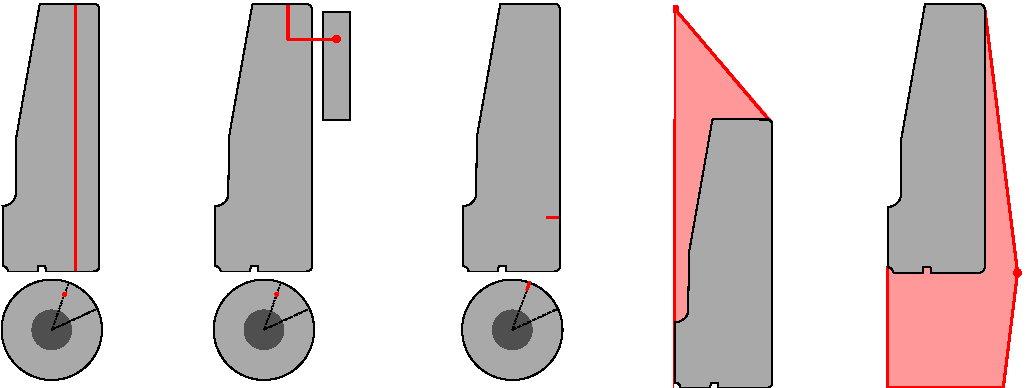
\includegraphics[width=6in]{figs/param/pictograms.pdf}
    \caption{Five pictograms representing data taken with the ICPC and \CsS{}, \BaS{} and \ThS{} sources.}
    \label{fig:pictograms}
\end{figure}

\noindent Going from left to right, the pictograms depict the following ICPC-source configurations. Note that where relevant cylindrical coordinates are given.
\begin{enumerate}
	\item Collimated \CsS{} source irradiating from the top at $(r_0,\phi_0)$ shown by the red line in the $\phi=\phi_0$ radial slice and red dot in the top view.
	\item Same as Pictogram 1, but only coincident events between the ICPC and camera are recorded. The camera and ICPC are shown to scale as is their relative $z$-position. However, the radial distance between the inner edge of the camera and the outer edge of the ICPC of 24.8\,mm is not shown to scale. 
	\item Collimated \BaS{} source irradiating from the side at position $(\phi_0,z_0)$ shown in the $\phi=\phi_0$ radial slice and top view. The much shorter range of \BaS{} gammas is illustrated with a short red line.
	\item Flood \ThS{} source placed concentric with the top of the ICPC, 14\,cm away. The distance between the top of the ICPC and the source is not shown to scale. 
	\item Flood \ThS{} source placed level with the p$^+$ contact and 9\,cm away from the outer edge of the ICPC. The distance between outer edge of the ICPC and source is not shown to scale. 
\end{enumerate}
The following is common to pictograms 1-3: The fast and slow axes of the ICPC are represented by dotted and dashed lines in the top view respectively. The following is common to pictograms 1-2: If data for more than 2 source positions is included in a figure, only the top view will show the source positions. If no source (red dots or lines) is shown on the pictogram, then it represents a background measurement. 

\section{Electronics Response}\label{sec:electronicsresponse}

The effects of the circuit shown in Fig.~\ref{fig:poptop_cicuit} are most succinctly observed in raw waveforms -- the output signals from the ADC -- as a baseline offset and exponentially decaying tail. These effects can be seen in Fig.~\ref{fig:baseline_removal} and Fig.~\ref{fig:decay_correction} respectively. The charge sensitive loop outputs an exponentially decaying signal with characteristic decay constant, $\tau_f = R_fC_f = 2$\,ms. The decay constant seen in data is the result of convolving this signal with the differentiator in the secondary amplification stage, which had a much sorter decay constant. 
%check tau with ORTEC

Prior to any waveform analysis, the baseline and tail decay were corrected. By fitting the first 1000 samples of a waveform to a line, the baseline offset ($B_o$) was calculated. In the low-event-rate regime, this value corresponds to a stable DC-offset (a resting baseline) on top of which signals evolve. However, higher rates drastically increase the probability that successive events occur before resting baseline conditions are restored. Although the decay is mostly governed by the second stage time constant, the convolution with the output of the charge sensitive loop introduces an undershoot from the DC-offset which recovers in the relatively long timescale characterized by $\tau_f$. Thus, as seen in Fig.~\ref{fig:baseline_removal}, the baseline offset distribution is highly asymmetric, with the events falling under the mode of the distribution resulting from this undershoot. The mode of the distribution provides a good estimate of the DC-offset. 
\begin{figure}[htb]
    \centering
    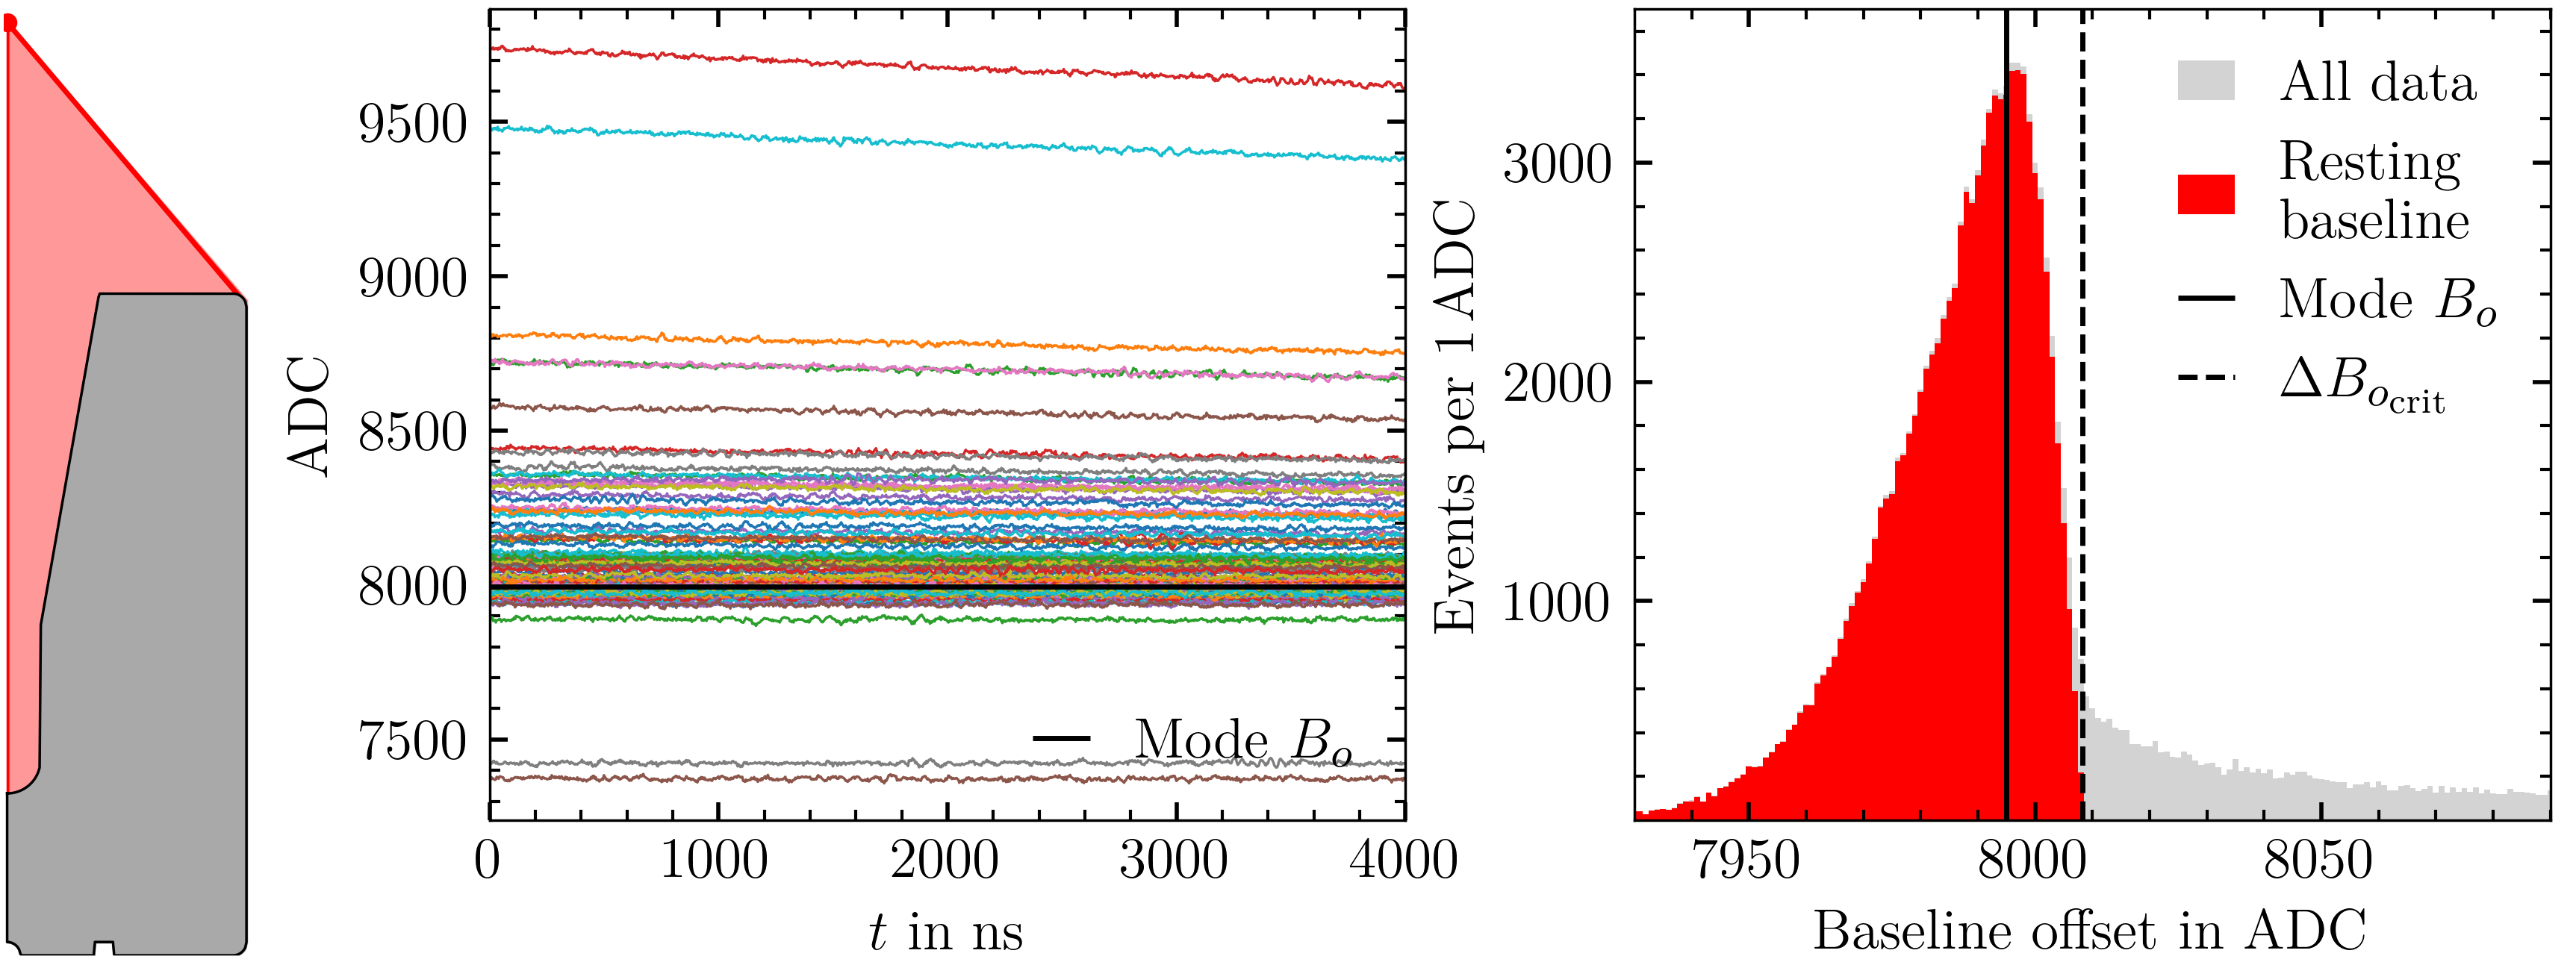
\includegraphics[width=6in]{figs/param/baseline_removal_6_9in.png}
    \caption{The first 1000 samples of 200 example raw waveforms (left) and baseline offset distribution (right). $\Delta B_o$, introduced in the next section, is a baseline offset value which is needed to construct a classifier for resting baseline events.}
    \label{fig:baseline_removal}
	\vspace*{-5pt}
\end{figure}

Meanwhile, events falling over the mode are categorized in two groups. If the slope from the linear baseline fit is significantly negative, the event likely occurred on the decaying tail of the previous event -- a soft pileup event. As the next section describes in detail, these events are categorized as soft pileup. On the other hand, events which do not have a slope which significantly deviates from zero, may still exhibit small fluctuations above the $B_o$ mode. Such events, along with those under the $B_o$ mode, are said to have a resting baseline. 

The baseline offset was calculated for all waveforms. For resting baseline events, the baseline offset can be directly subtracted. An example baseline subtracted event is shown in Fig.~\ref{fig:decay_correction}. After baseline offset subtraction an exponential function was fit to the central 4$\upmu$s portion of the tail of each waveform to calculate the decay constant. As opposed to the baseline offset, this value is very stable, and a single decay constant was used to correct all waveforms. Pileup-free waveforms in the 2615\,keV $^{208}$Tl FEP of a \ThS{} calibration were originally used to calculate this parameter. This population of events was chosen due to the high signal-to-noise ratio. The resulting $55.35\,\upmu$s decay constant -- once employed in decay correcting all waveforms -- created undesirable correlations between baseline slope and decay corrected (residual) baseline slope in soft pileup events. In an effort to correct this, longer waveforms were employed for decay constant estimation: the approximately 260\,$\upmu$s long waveforms recorded during noise characterization. 
\begin{figure}[htb]
    \centering
    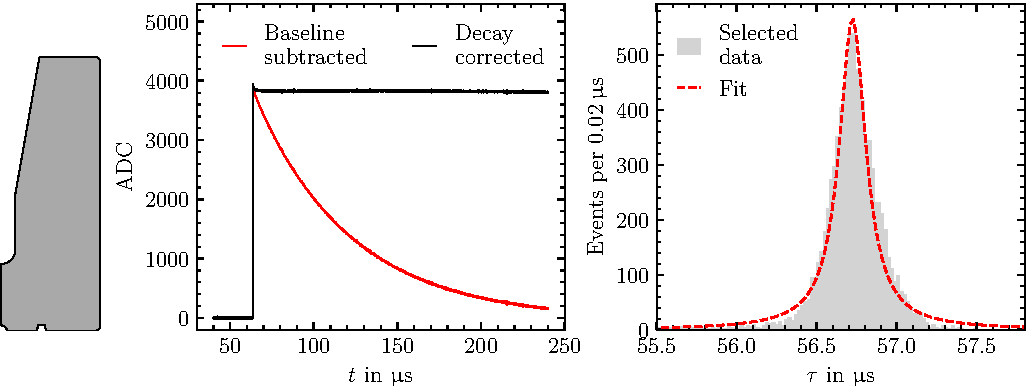
\includegraphics[width=6in]{figs/param/decay_correction_longwf_6_9in.pdf}
    \caption{An example waveform from noise characterization is decay corrected with the decay constant, $\tau$, calculated from the Cauchy fit to the distribution on the right.}
    \label{fig:decay_correction}
\end{figure}

Although no calibration source was used, approximately 10,000 pileup-free waveforms over 400\,keV were found in the data. Using the 100\,$\upmu$s window starting at 4\,$\upmu$s after the waveform achieved 50\% of its maximum, a decay constant of $(56.72 \pm 0.10)\,\upmu$s was obtained. The unbinned Cauchy fit shown in Fig.~\ref{fig:decay_correction} was used to extract this parameter and its error, which represents half of the FWHM of the distribution. This decay constant was used to correct all the waveforms, regardless of the DAQ mode used. Although smaller evaluation windows close to the maximum of the waveform and toward the end of the decay result in decay constants 2-3\% smaller, the chosen decay constant results in the best energy resolution. The different time constants calculated encapsulate the effect of the coupling between different time constants in the electronics chain. The analysis is simplified by the use of one time constant, which corrects for most of the decay and is suitable for the range of event rates in the data taken.

The electronics also shape the waveforms in more subtle ways. To introduce these effects in simulated waveforms, the electronics response function is needed. This function is simply the normalized output of the current signal to a step function input. A pulse generator was connected to the pulser line of the PopTop for this purpose. The waveforms resulting from 50\,mV step pulses are shown in Fig.~\ref{fig:electronics_response}. 
\begin{figure}[htb]
    \centering
	\vspace*{-10pt}
    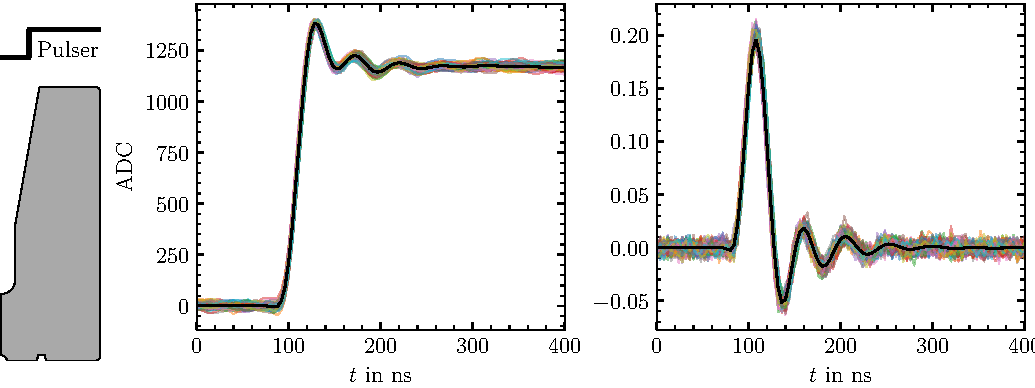
\includegraphics[width=6in]{figs/param/electronics_responce_6_9in.pdf}
	\vspace*{-10mm}
    \caption{100 example response waveforms and the response superpulse (left) used to calculate the response function in black on the right.}
    \label{fig:electronics_response}
	\vspace*{-5pt}
\end{figure}

Background events were removed from pulser data by enforcing that the time between pulser events matches that of the pulse generator period. All the events passing this timing cut are used to construct a superpulse. To do so, the waveforms are aligned at 50\% of their rise and averaged sample by sample. The use of 70,000 events drastically reduces the noise. The superpulse is decay corrected, its derivative is taken, and the result is normalized to produce the electronics response function shown on the right in Fig.~\ref{fig:electronics_response}. Simulation of the electronics chain can be achieved by convolving simulated waveforms with this function. In data, the effects of the electronics response function are most saliently represented by an overshoot from the decay corrected waveform tail.  

\section{Pileup Classifiers and Corrections} \label{sec:pileup}

Pileup probability is governed by Poisson statistics and depends on the activity and proximity of the source, and the volume and decay constant of the detector. Given the high activity of the \CsS{} source and the large volume of the detector, a significant amount of pileup is expected. Hard pileup occurs when both events fall within the same waveform window. On the other hard, only the decaying tail of the previous event remains in the waveform window of a soft pileup event, thus this type of pileup can be identified by searching for baselines with negative slopes.

The baseline slope was extracted from the linear fit to the first 1000 samples of the waveform described in the previous section. The slope is defined here as the ADC shift after 1000 samples. In reality, the baseline is exponentially decaying for soft pileup events. However, in the 1000 sample (4\,$\upmu$s) window, a fairly linear behavior is observed, and thus the slope is appropriate for soft-pileup identification purposes. 
\begin{figure}[htb]
    \centering
    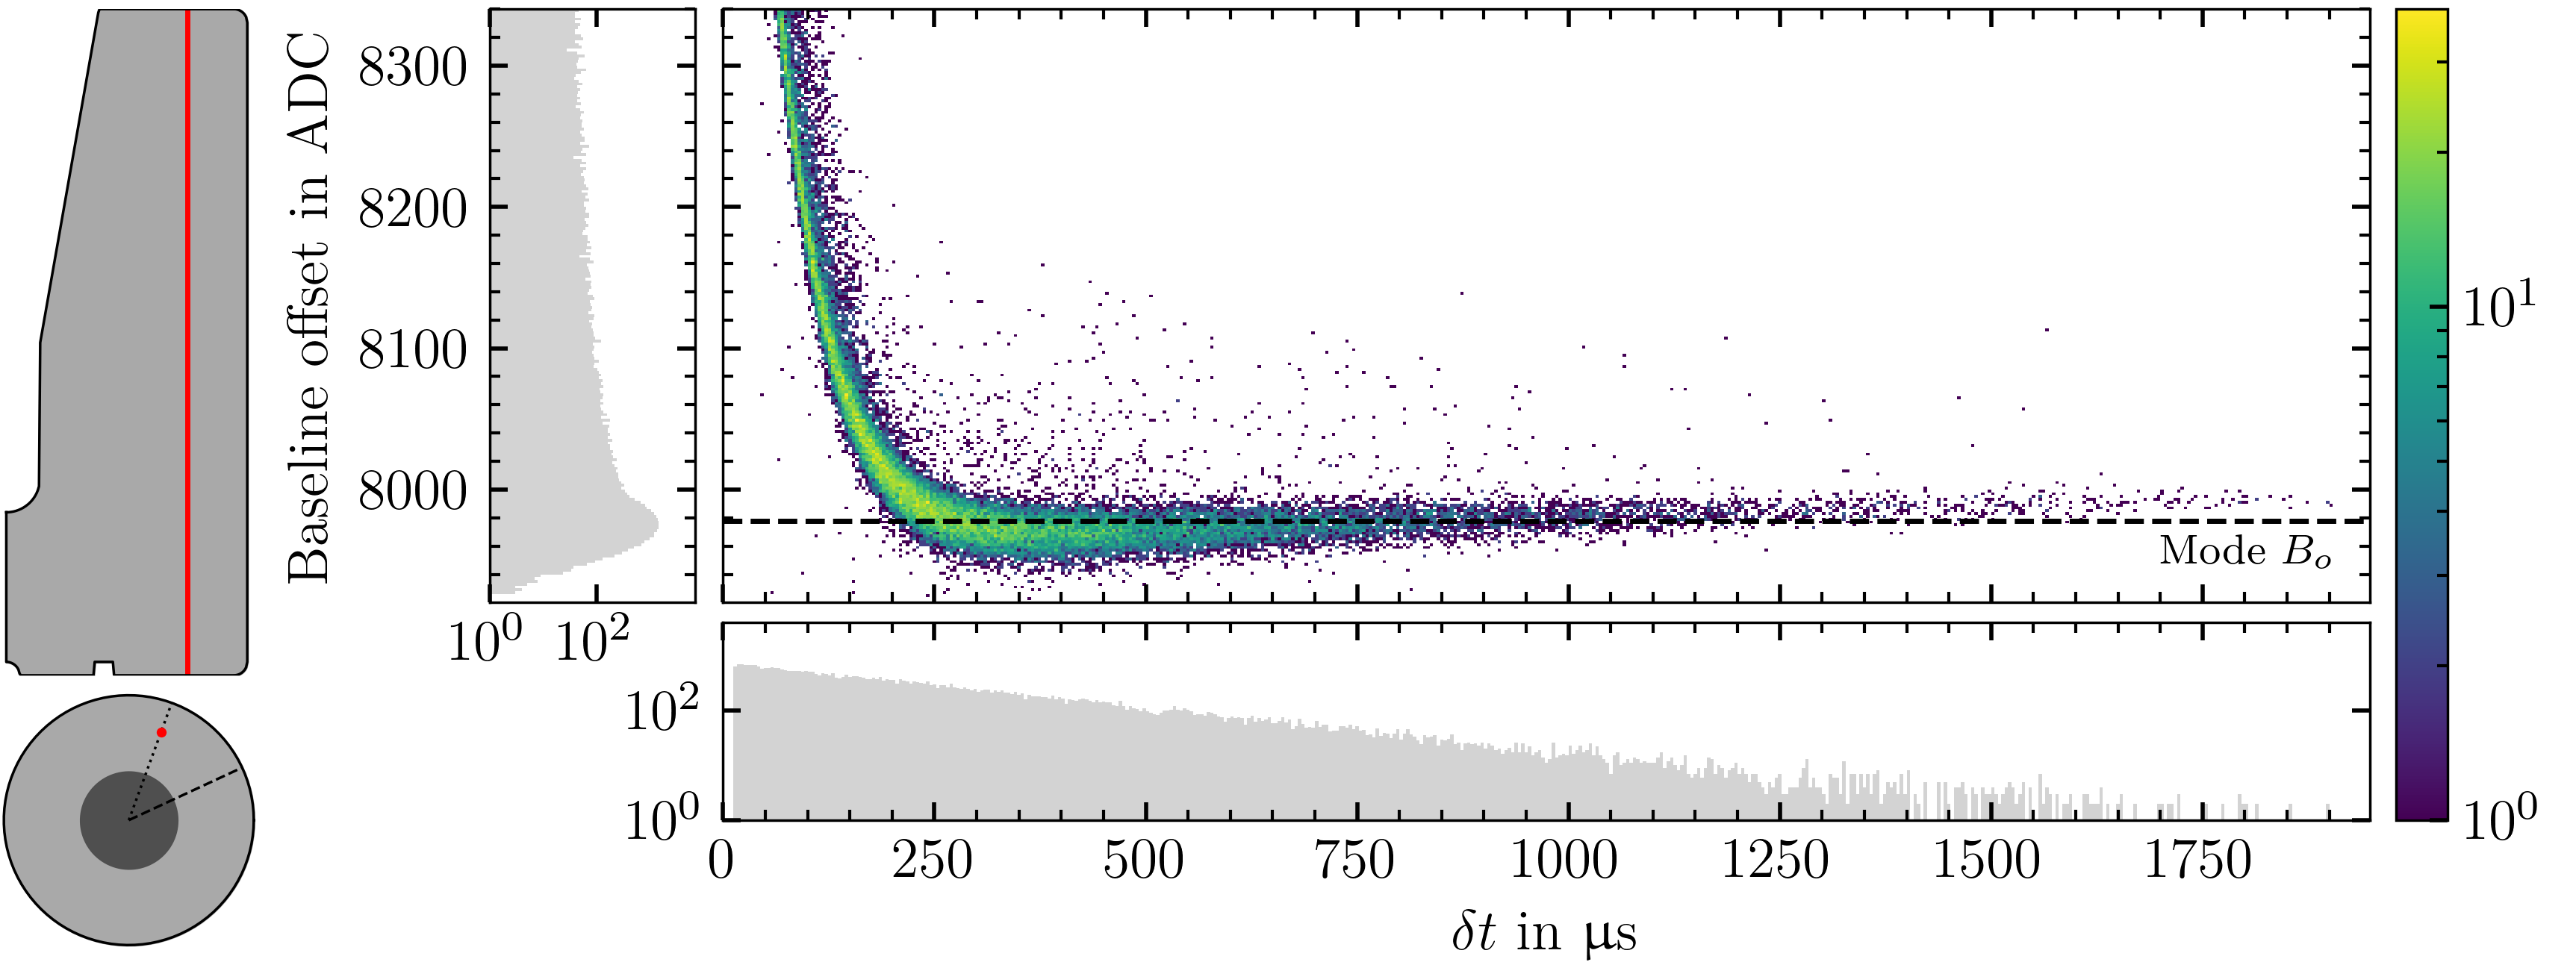
\includegraphics[width=6in]{figs/param/dt_offset_maginalized_6_9in.png}
    \caption{An average 662\,keV event waveform tail is generated as described in the text. The marginalized distributions of $\delta t$ (difference between event DAQ trigger times) and baseline offset are shown in the margins. $\delta t$ follows the expected exponential distribution obtained from the 3.3\,kHz event rate.}
    \label{fig:time_vs_offset}
\end{figure}

The baseline offset and slope depend on the time elapsed since ($\delta t$) and the energy of the previous event. By plotting the baseline offset against $\delta t$ for all events following a FEP event -- say 662\,keV for a \CsS{} measurement -- an average shape of the tail of FEP waveforms can be constructed. As seen in Fig.~\ref{fig:time_vs_offset}, and described in the previous section, waveforms decay with a 56.72\,$\upmu$s decay constant, produce a small undershoot and recover in the time characterized by the decay constant of the charge sensitive loop. The baseline slope is simply the derivative of the trend observed in this plot. 

$\delta t$ can act as a powerful discriminator for soft pileup events. However, its use requires a near-zero dead time, and for the time of the previous event to be saved. Neither of these conditions is met when coincidence filtering is turned on (Compton DAQ mode), therefore the correlation between baseline slope and offset is used instead. Also note that a $\delta t$ would necessarily be energy dependent. The distribution of the slope and offset is shown in Fig.~\ref{fig:soft_pileup} for data collected with the \CsS{} source over one of the detector's arms, 27\,mm from the center of the detector. The highest trigger rates are expected in this region and consequentially, the highest soft (and hard) pileup rates. The trigger rate in the center of the detector is 35\% lower, which matches the estimation from attenuation lengths.  
\begin{figure}[htb]
    \centering
    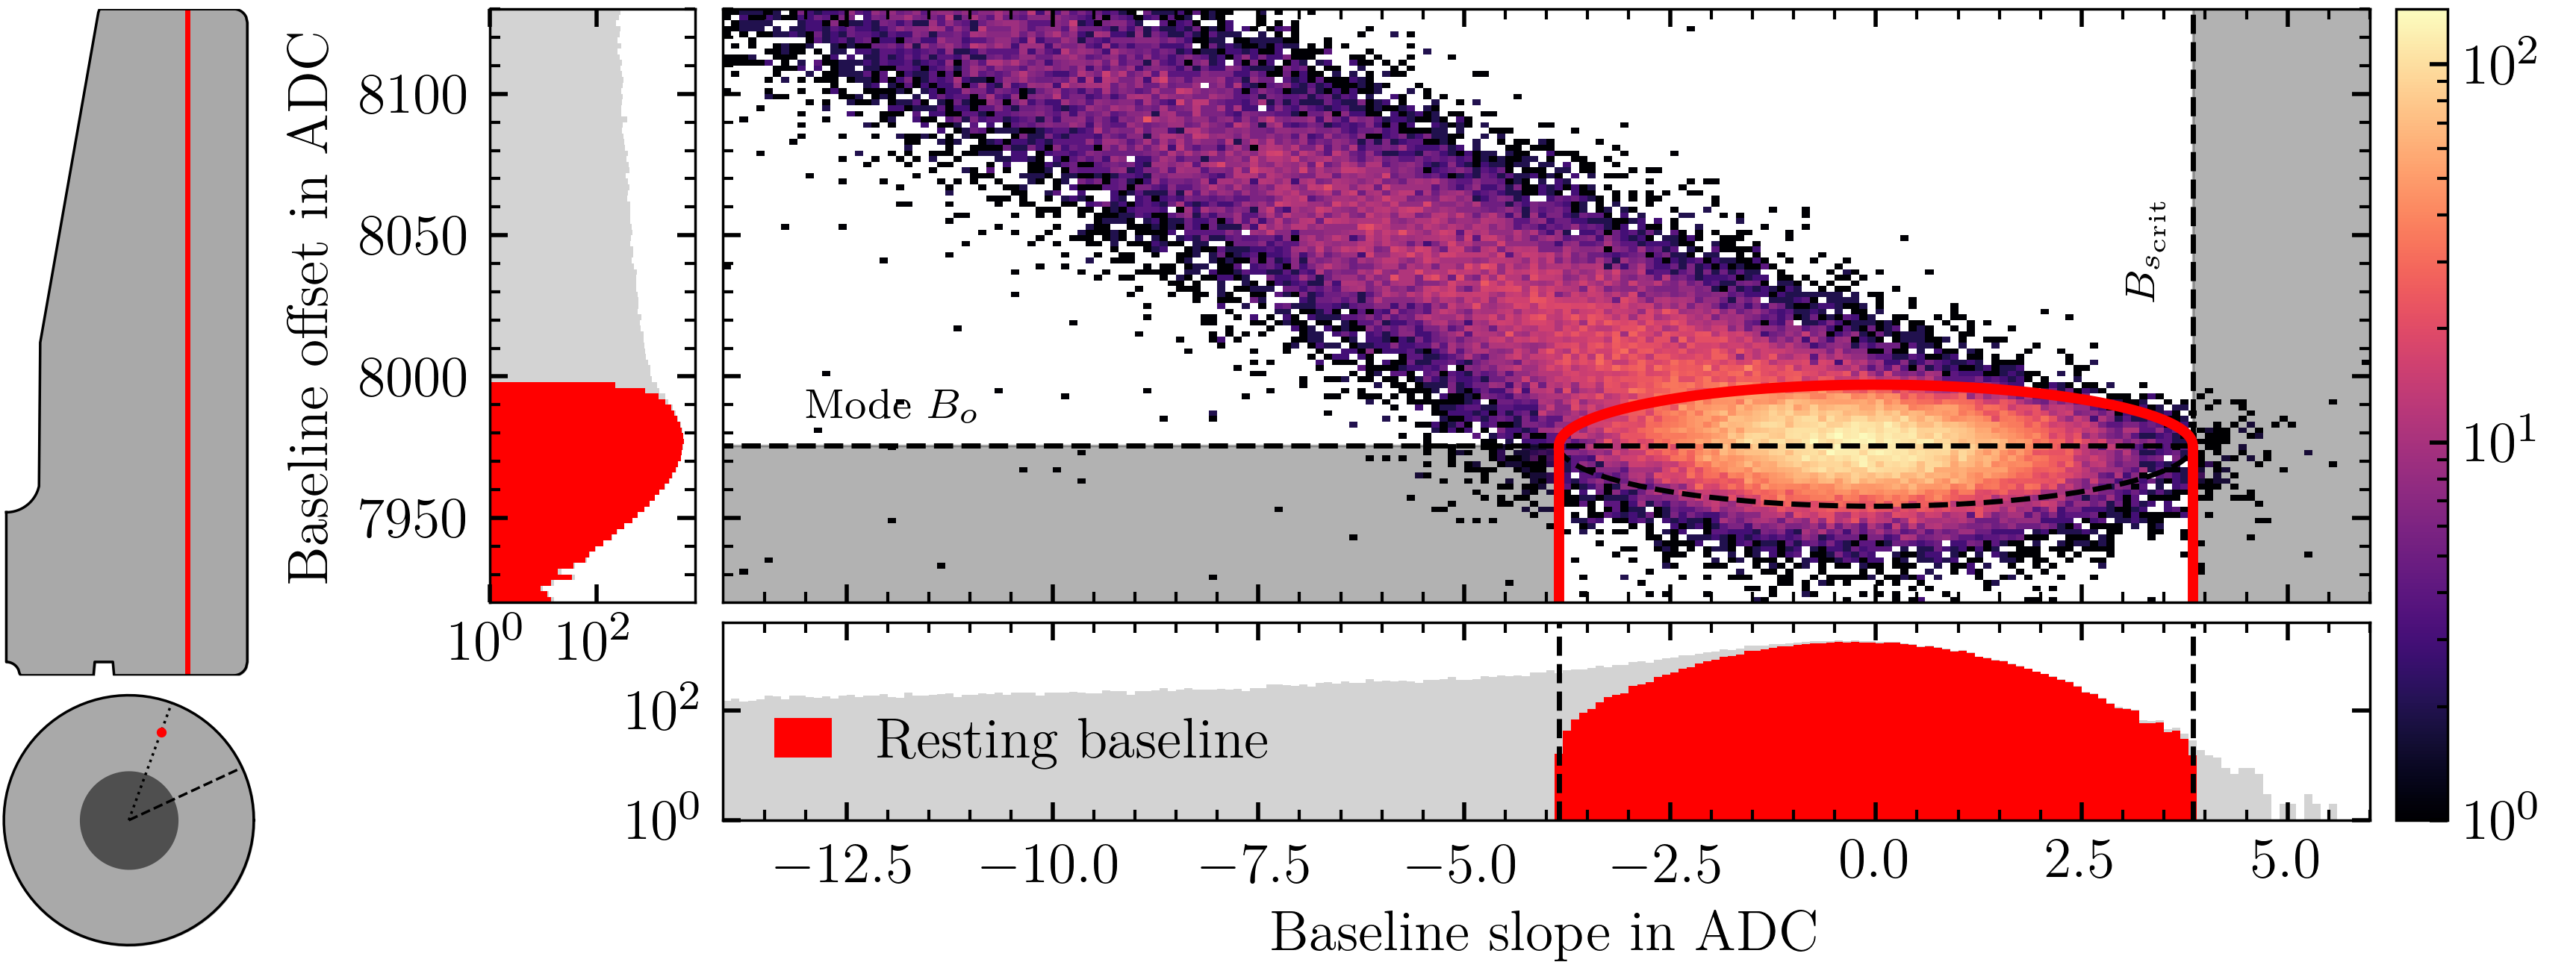
\includegraphics[width=6in]{figs/param/soft_pileup_maginalized_6_9in.png}
    \caption{Representation of soft pileup classification procedure described in the text.}
    \label{fig:soft_pileup}
\end{figure}

From Fig.~\ref{fig:time_vs_offset}, it is clear that most events with baseline offset under the $B_o$ mode have achieved resting baseline conditions. The problem lies in identifying resting baseline events over the mode. For this purpose the correlation with the baseline slope was used. Events under the mode were used to construct a slope interval in which most resting baseline events should lie. Three times the 84.1$^\text{th}$ slope percentile set the upper cut value, $B_{s_\text{crit}}$. This is equivalent to at 3$\sigma$ cut of a symmetric Gaussian centered at zero. The baseline slope distribution of events of the chosen population closely resembles such a distribution. Assuming a symmetric distribution of resting baseline slope, this cut value was reflected over zero to construct the slope interval for resting baseline events. If this interval is applied to events over the mode, a considerable amount of soft pileup events are retained, as seen in as the gray excess (above the red) in the marginalized slope distribution in Fig.~\ref{fig:soft_pileup}. To resolve this issue, a new parameter -- the baseline ``radius'' -- was created. The definition follows: 
\begin{equation}
	B_r^2 \equiv \frac{(B_o - \text{mode}(B_o))^2}{\Delta B_{o_\text{crit}}^2} + \frac{B_s^2}{B_{s_\text{crit}}^2}
	\label{eq:baseline_radius}
\end{equation}
where $B_r$, $B_o$ and $B_s$ are the baseline radius, offset and slope respectively which are calculated from each waveform. The critical deviation from $B_o$ mode, $\Delta B_{o_\text{crit}}$, was calculated as twice the difference between the 68.3$^\text{th}$ percentile of events with slopes above zero and offsets above the baseline mode, and the baseline mode. The calculation of this value, along with $B_{s_\text{crit}}$ and the $B_o$ mode, requires on the order of 500 or more waveforms. Thus, they were calculated every 5 min, using the data collected in each time interval.

$B_r^2 = 1$ constitutes an ellipse enclosing resting baseline events. Thus, events with $B_r^2\le1$ are flagged as having a resting baseline. Events with $B_r^2>1$, $B_o < \text{mode}(B_o)$ and $\|B_s\| \le B_{s_\text{crit}}$ are also included in this population. Together they constitute the area in slope-offset space enclosed by the red curve in Fig.~\ref{fig:soft_pileup}. This classifier was successful at recovering more symmetric slope and offset distributions for resting baseline events. These are seen as the red areas in the marginalized distributions. Note that the cuts also eliminate the tail of these distributions, on one side or both. All events falling in the dark gray regions -- less than 1\% -- are flagged as abnormal and discarded. Finally, events falling in the non-shaded region above the red curve are flagged as soft pileup, which constitutes 55\% of the data in this measurement. 

Events following a FEP \CsS{} event, such as those used in Fig.~\ref{fig:time_vs_offset} can be used to test the performance of the soft pileup classifier. As the rightmost panel of Fig.~\ref{fig:soft_pileup_eval} shows, almost all resting baseline events fall above four times the decay constant after the previous event, approximately where the average 662\,keV event tail of Fig.~\ref{fig:time_vs_offset} crosses the baseline mode. Additionally, little soft pileup contamination exits above this value. The latter is not the case of single-parameter classifiers. The left panel of Fig.~\ref{fig:soft_pileup_eval} shows the result of using $B_s < 0$ to select soft pileup events.
\begin{figure}[htb]
    \centering
    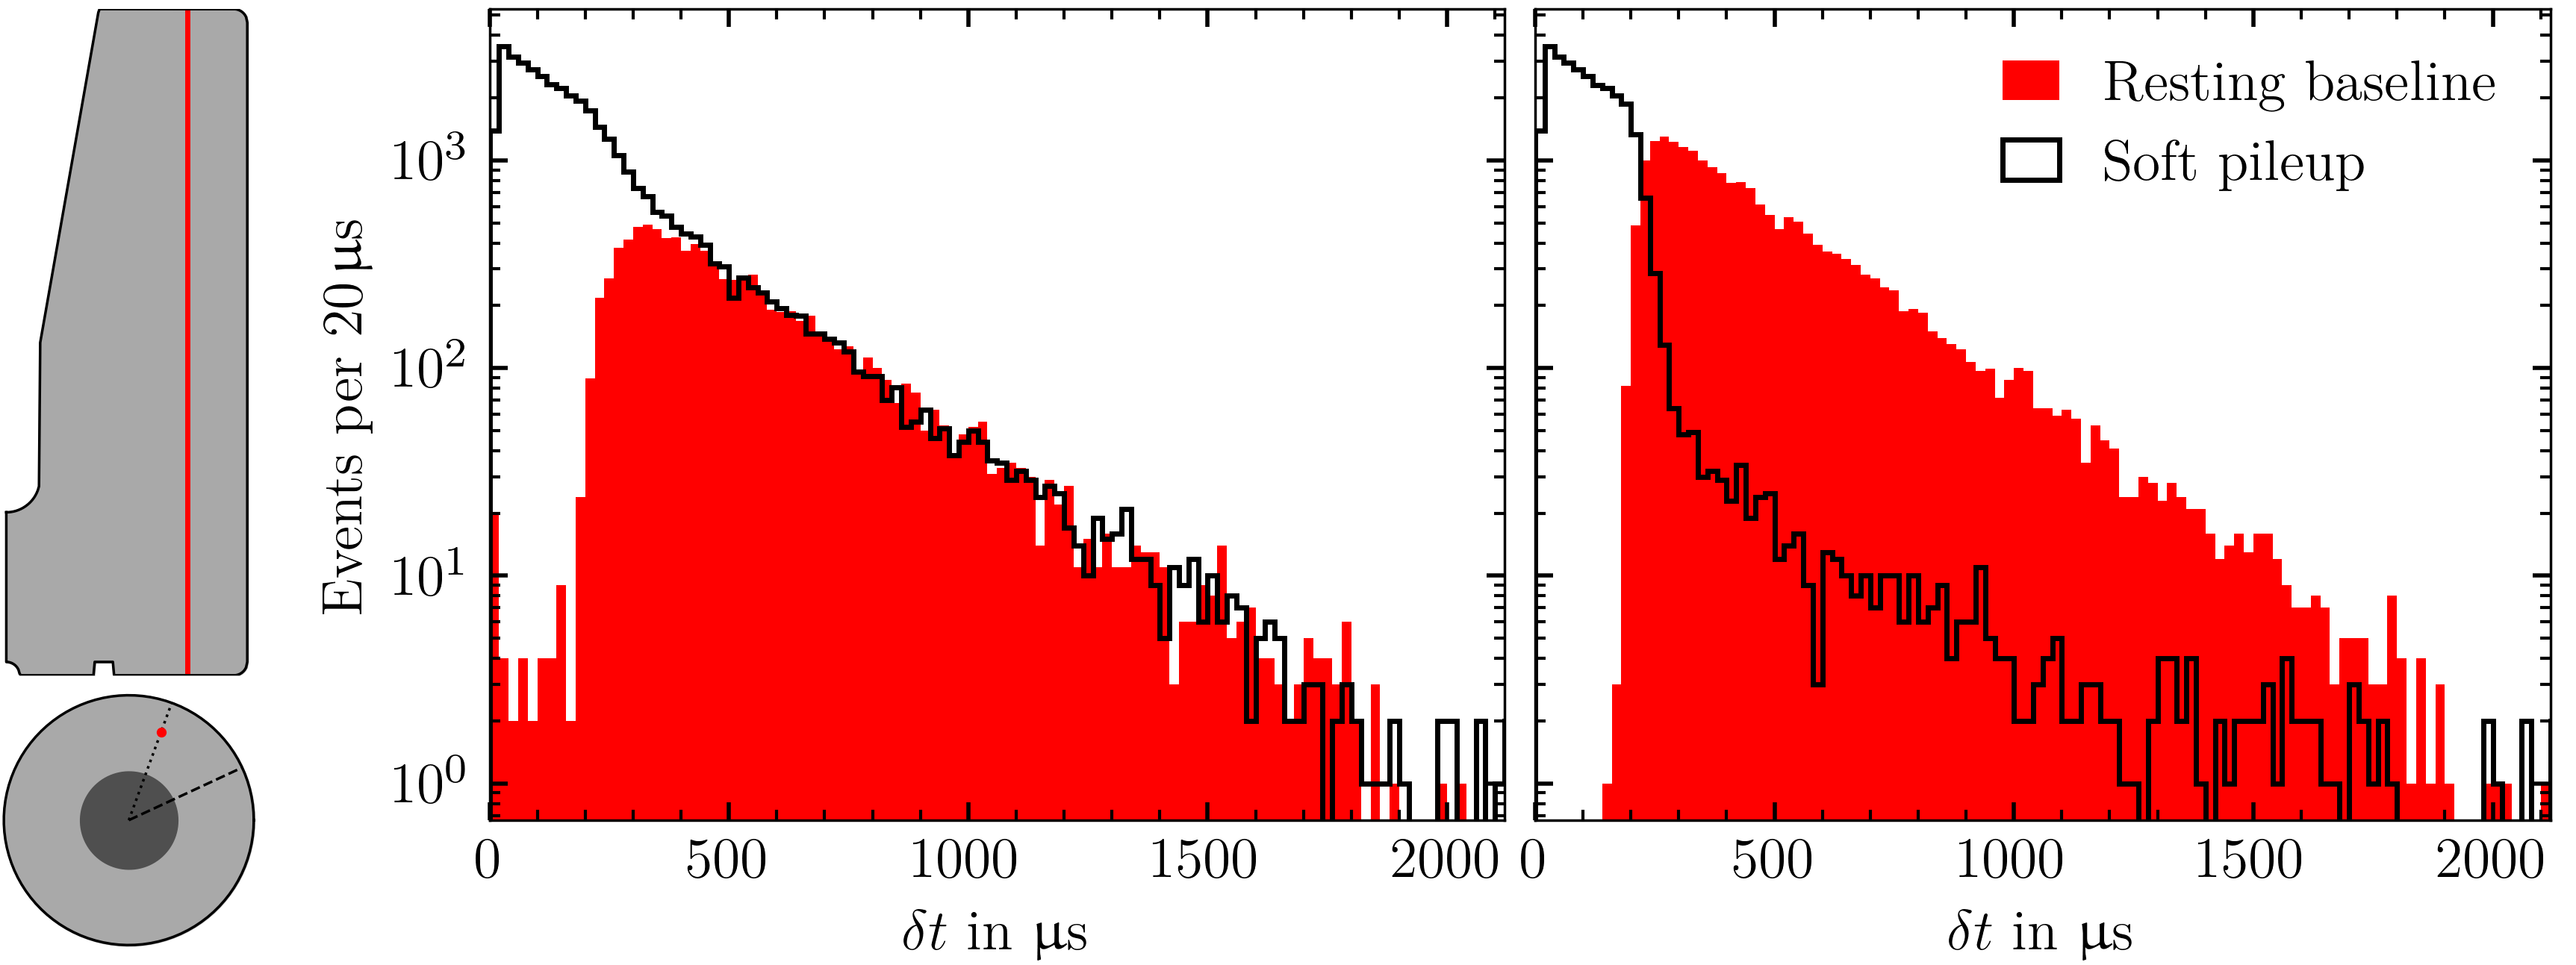
\includegraphics[width=6in]{figs/param/dt_pileup_classifier.png}
    \caption{$\delta t$ distribution for resting baseline and soft pileup events for the $B_s < 0$ classifier (left) and the multi-parameter classifier described in the text (right).}
    \label{fig:soft_pileup_eval}
\end{figure}

The performance and stability of the soft pileup classifier was analyzed during Compton and Germanium mode data over months of data taking by periodically inspecting slope-offset plots, such as that in Fig.~\ref{fig:soft_pileup}. The baseline offset parameters in Eq.~\ref{eq:baseline_radius} are shown over time for a full Compton radial scan in Fig.~\ref{fig:baseline_stability} 
\begin{figure}[htb]
    \centering
    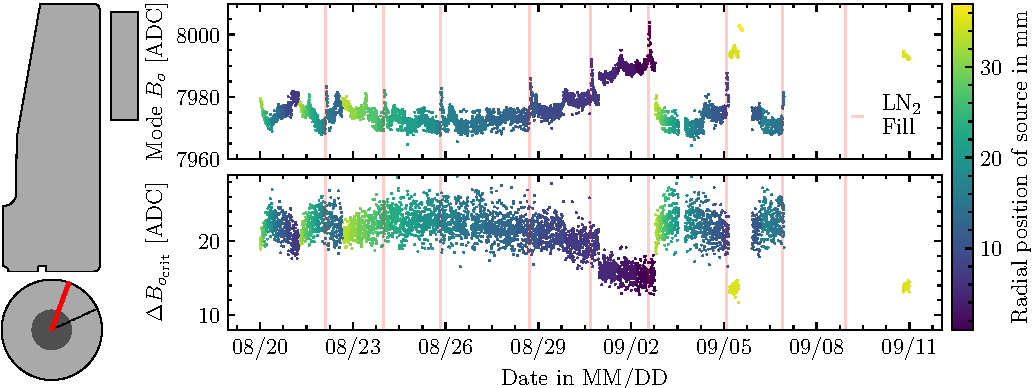
\includegraphics[width=6in]{figs/param/baseline_stability.pdf}
    \caption{$B_o$ mode and critical deviation from $B_o$ mode ($\Delta B_{o_\text{crit}}$) for one Compton radial scan. Spikes in the $B_o$ mode are caused by LN$_2$ fills. While the fill only last 3 minutes, the $B_o$ mode takes around 3 hours to settle. Due to the rate difference, the position of the source also affects the $B_o$ mode. Most notably, when the source is at the outer edge of the detector (yellow), $B_o$ modes are usually higher, and deviations from this value are considerably lower. At this source position the beam spot is half-off the detector, leading to the lowest rates of the radial scan.}
    \label{fig:baseline_stability}
\end{figure}

Instead of discarding the flagged soft pileup events, the waveforms were corrected with the decay correction introduced in Sec.~\ref{sec:electronicsresponse}. The $B_o$ mode is used in a first round of baseline subtraction. The $B_o$ mode subtracted waveforms were then decay corrected, and any final offset from zero was subtracted. As seen in Fig.~\ref{fig:soft_pileup_corr}, near total baseline slope correction was achieved with this procedure, with very little correlation between baseline slope and residual baseline slope. The residual baseline slope distribution is Gaussian, with a slightly negative mean. This shift is caused by the faster decay time at the end of the waveform tails.  
\begin{figure}[htb]
    \centering
    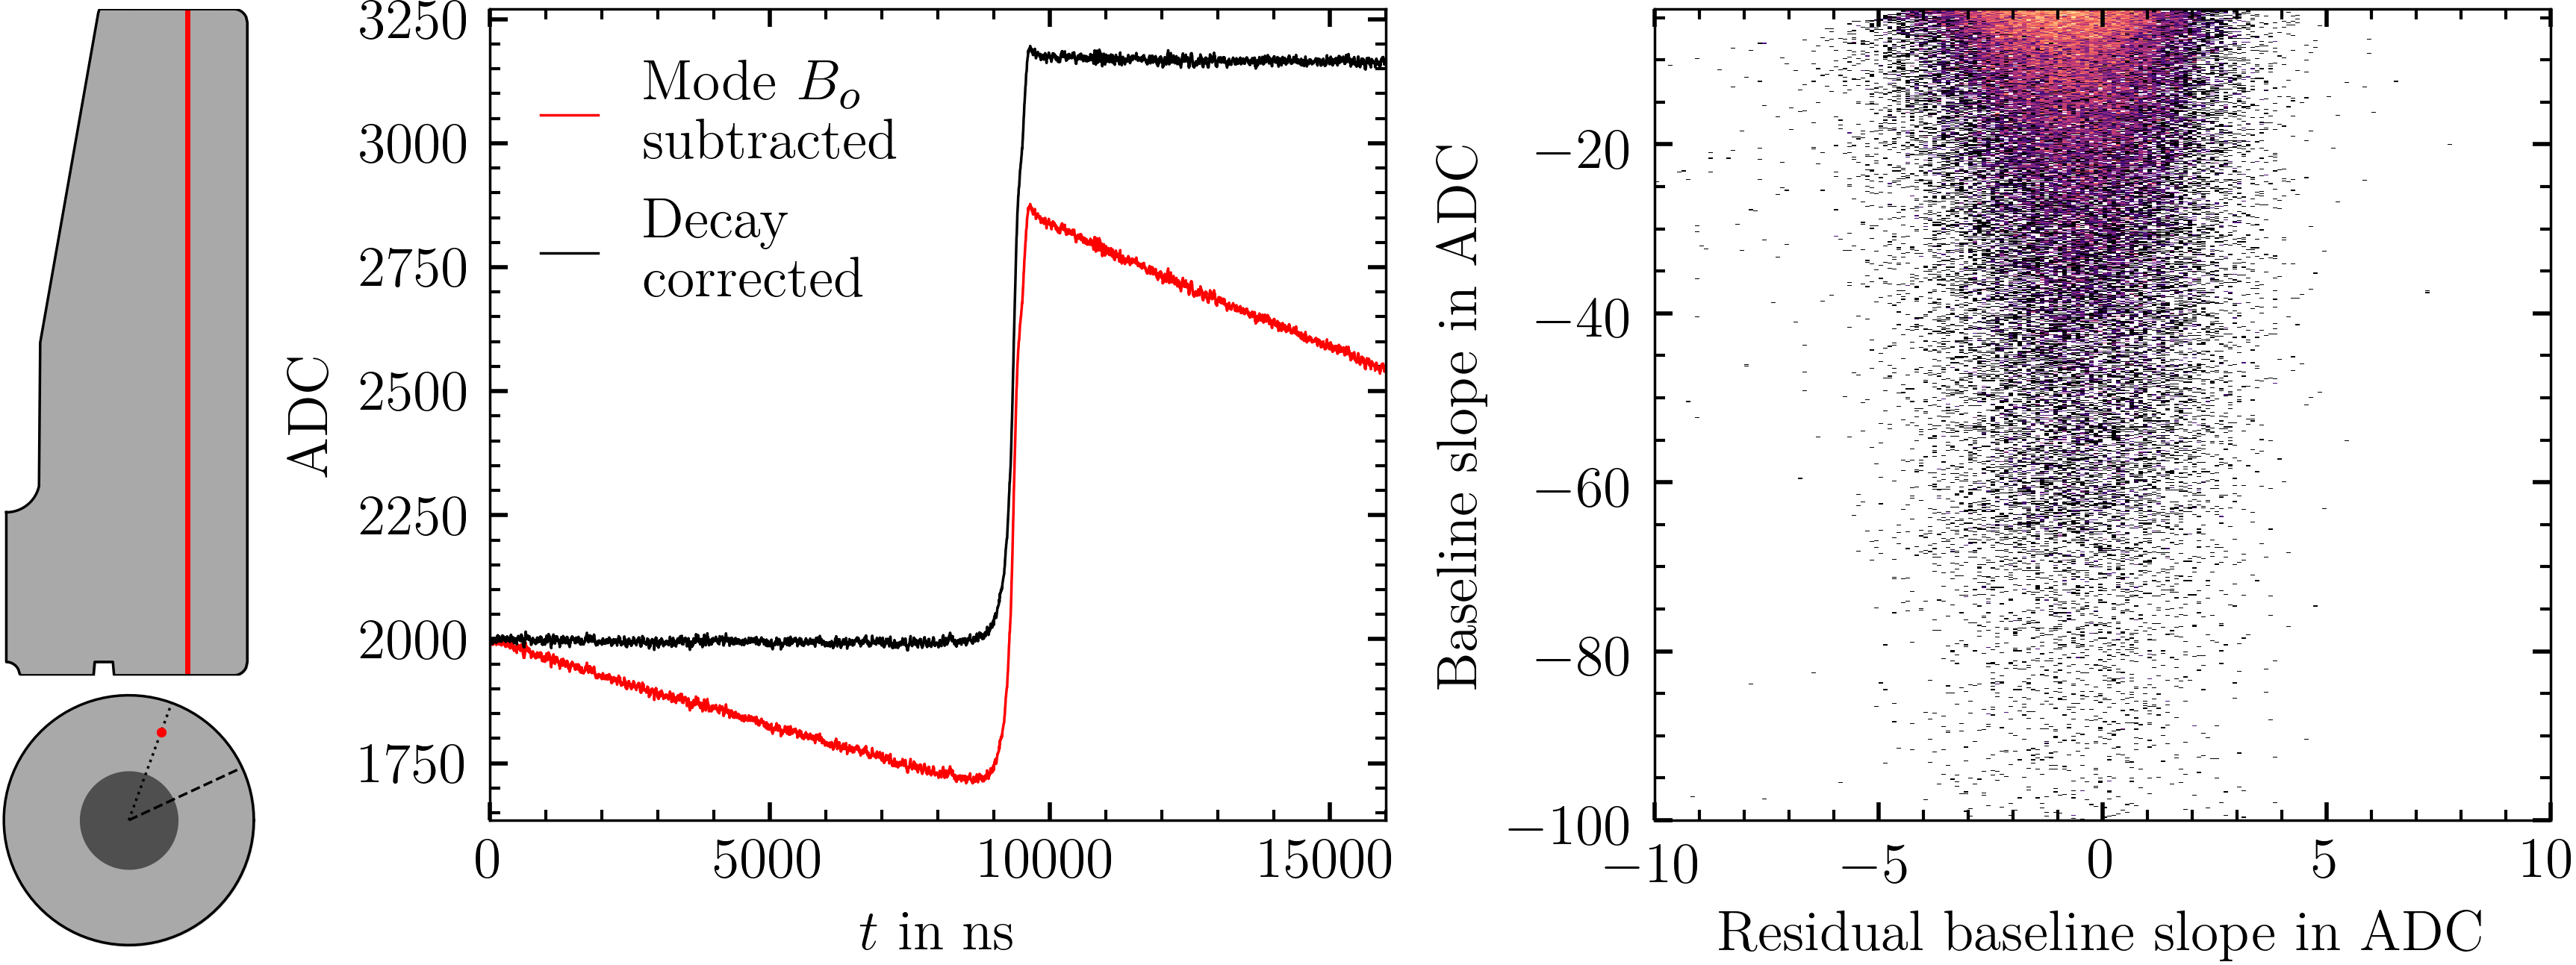
\includegraphics[width=6in]{figs/param/soft_pileup_corr_6_9in.png}
    \caption{An example soft pileup waveform and its correction (left) and the residual baseline slope distribution of the corrected waveforms (right).}
    \label{fig:soft_pileup_corr}
\end{figure}

Since waveforms with soft pileup and without require different corrections, two parallel waveform analysis pipelines were created: 
\begin{enumerate}
	\item Resting baseline waveforms were baseline-offset-removed-decay-corrected (BRDC)
	\item Soft pileup waveforms were baseline-offset-mode-removed-decay-corrected (MRDC)
\end{enumerate}
In all cases, the resting baseline event parameters that follow are calculated on BRDC waveforms, and conversely, soft pileup event parameters are calculated on MRDC waveforms. 

The identification of hard pileup is more straight forward. A trapezoidal filter with rise-flat-fall time of 0.2\,$\upmu$s-1.4\,$\upmu$s-0.2\,$\upmu$s was applied to each waveform. If the number of rising threshold crossings of the trapezoidal transformed waveform is greater than one, and such crossings are further than 1.4\,$\upmu$s apart, then a hard pileup flag is placed on the event. The 0.2\,$\upmu$s rise or integration time of the pileup trapezoid was chosen such that a 10\,ADC threshold does not pick up noise. The sum of the pileup trapezoid parameters sets a minimum trapezoidal width of the filtered waveforms of 1.8\,$\upmu$s. However, since most waveforms are not step-like, trapezoidal widths are closer to 2.5\,$\upmu$s, effectively ensuring that detector hits in hard-pileup flagged events are slightly over the maximum drift time apart. The soft-pileup-removed \CsS{} energy spectrum is shown in Fig.~\ref{fig:hard_pileup}. Events flagged as hard pileup are shown in red. 

\begin{figure}[htb]
    \centering
    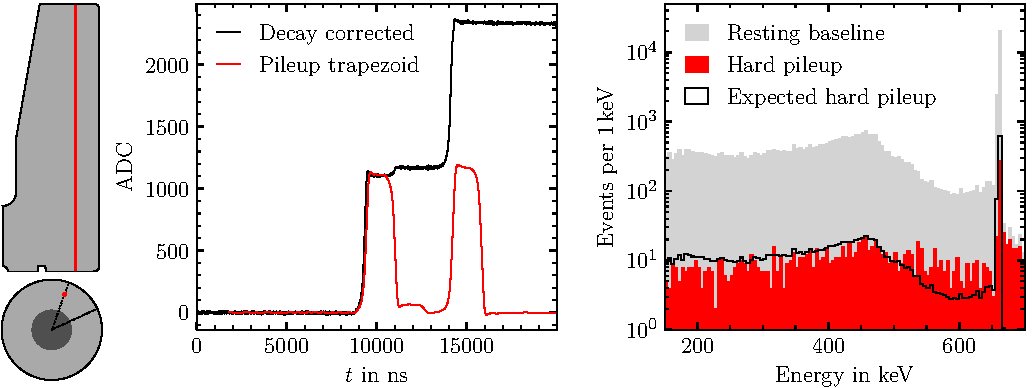
\includegraphics[width=6in]{figs/param/hard_pileup_6_9in.pdf}
    \caption{An example hard pileup waveform is identified by the application of a trapezoidal filter with the appropriate parameters (left). The measured \CsS{} spectrum (gray) is used to determine the expected hard pileup. The hard pileup identified by the trapezoidal discriminator is shown in red (right).}
    \label{fig:hard_pileup}
\end{figure}
The time between detector hits, $\delta t$, follows an exponential distribution with the decay constant corresponding to the count rate of the detector, $r$. Therefore, by integrating this distribution over the $\delta t$'s that the hard pileup is sensitive to, the expected hard pileup fraction, $f_\text{hp}$, can be estimated. 
\begin{equation}
	f_\text{hp} = \int_{2.5\,\upmu s}^{12\,\upmu s}re^{-r\delta t}d\delta t 
	\label{eq:expected_pileup}
\end{equation}
Where 12\,$\upmu$s is the length of the waveform after triggering. In Fig.~\ref{fig:hard_pileup}, the soft-pileup-removed energy spectrum is scaled by $f_\text{hp}$ to produce the expected hard pileup spectrum. Due to the 4.5\,$\upmu$s integration time used in energy estimation (Sec.~\ref{sec:energy}), hard pileup shifts energies towards higher values. Thus, more events than expected are tagged above the Compton shoulder and FEP of \CsS{}. In the data shown, 3.4\% of resting baseline events are flagged as hard pileup, a figure close to that calculated from Eq.~\ref{eq:expected_pileup}, 3.1\%. Unless otherwise stated, hard pileup is removed prior to all analyses. 

\section{Noise Burst Classifier}
Due to the presence of the rising edge, the parameter previously used to determine noise amplitude, $B_w(1000)$, cannot be used in the signal window to discriminate against bursts. However, the burst structure observed in Fig.~\ref{fig:burst_waveforms} and Fig.~\ref{fig:long_trace} can be exploited to remove events with bursts in the signal window. Each burst consists of at least four prominent minima. By taking the derivative of the waveforms -- the current -- bursts may be observed along the entire signal window, including the rising edge, as repeated prominent negative spikes. It is hard to distinguish these from the overall noise of the current. Therefore, a moving window average (MWA) of the current is taken to increase the difference between the negative amplitude of the noise and the bursts. A window of approximately half the burst period (44\,ns) maximizes this effect. 
\begin{figure}[htb]
    \centering
    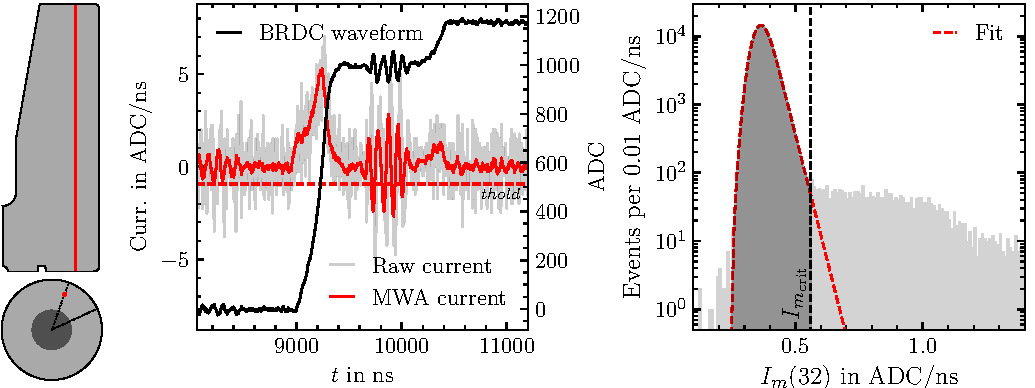
\includegraphics[width=6in]{figs/param/current_min_fit_6_9in.pdf}
    \caption{$I_m(32)$ is calculated as described in the text and exemplified on the left panel to produce the $I_m(32)$ distribution of Compton data shown on the right. The distribution is fit to the high-energy-tail version of the response function of Eq.~\ref{eq:energy_peak_fit}. to determine $I_{m_\text{crit}}$.}
    \label{fig:current_min_burst}
\end{figure}

A new burst discriminator, named $I_m(32)$, is obtained by taking the mean of the 32 lowest ADC values of the MWA current. This process is visualized in the left panel of Fig.~\ref{fig:current_min_burst}, where the 32 samples below the threshold are averaged. The minimum MWA current can also be used, but it was empirically found that using 32 samples led to a greater rejection of bursts. The resulting $I_m(32)$ distribution of Compton data taken during the main measurement campaign is shown on the right of the same figure.

Similar to the baseline width cuts, a cut value -- $I_{m_\text{crit}}$ -- was set such that 99.9\% of the fitted peak is retained. By comparing the number of events with $I_m(32) > I_{m_\text{crit}}$ to the number of bursts expected -- given by $B_w(1000)$ -- it is estimated that 78.1\% of bursts in the signal window are rejected. This cut retains approximately 97.7\% of Compton mode data.

The performance of the burst classifier was evaluated at higher energies than those in Compton mode, i.e. above 662\,keV during \ThS{} energy calibrations. 
\begin{figure}[htb]
    \centering
    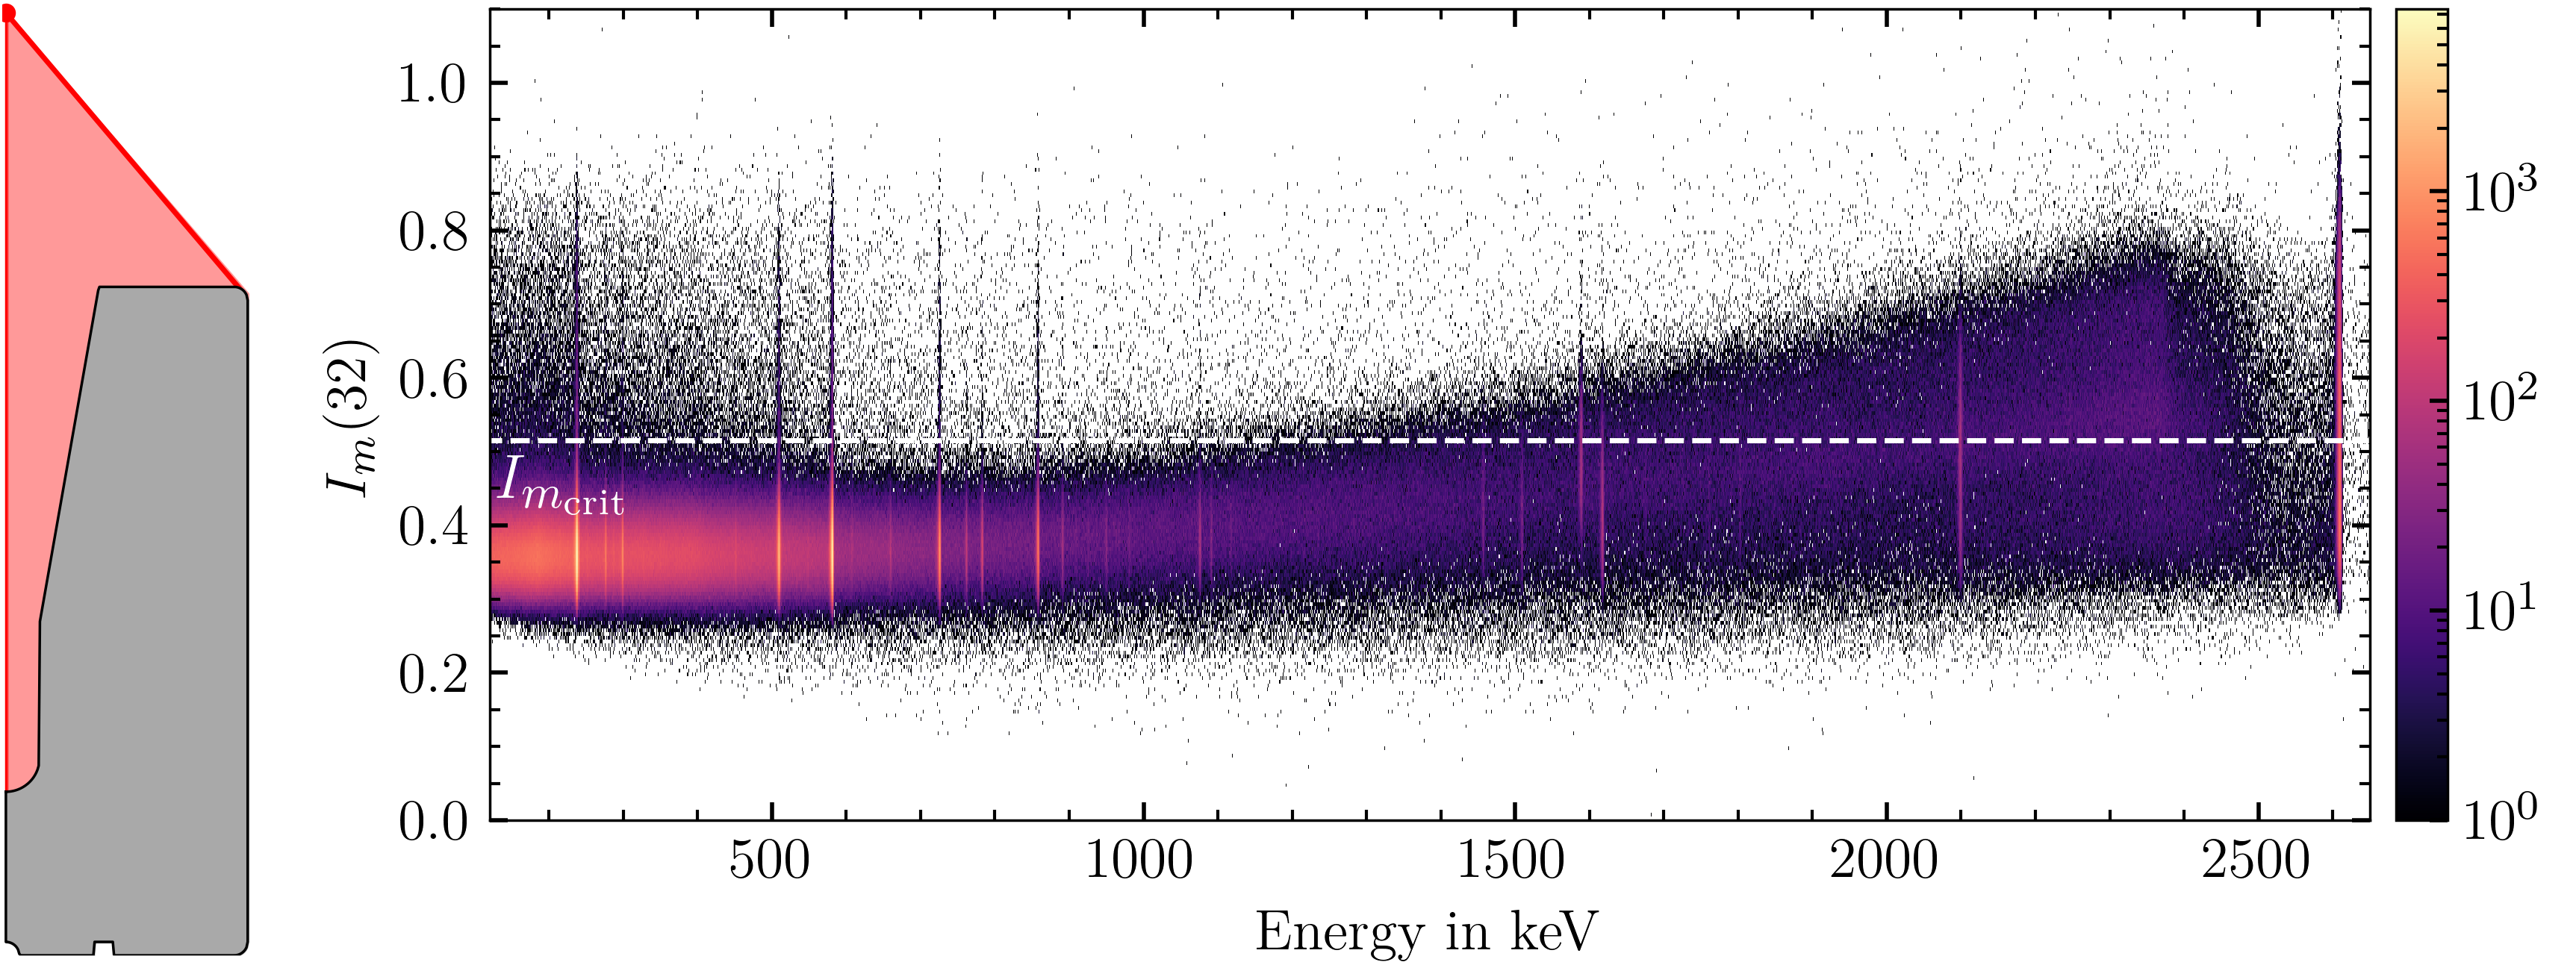
\includegraphics[width=6in]{figs/param/Im32_spectrum_6_9in.png}
    \caption{\ThS{} calibration $I_m(32)$ distribution. $I_{m_\text{crit}}$ is calculated for energies below 662\,keV and shown as a dashed white line. Note that this value is slightly smaller than in Compton data, due to the Camera system being shut off during \ThS{} energy calibrations.}
    \label{fig:current_min_spectrum}
\end{figure}
The more pronounced effect of the electronics response model above 900\,keV induces negative current right after the full rise of a waveform, obscuring the effects of bursts. This effect can be seen as a shift and broadening of the $I_m(32)$ distribution above this energy in Fig.~\ref{fig:current_min_spectrum}. Therefore, the burst cut was only applied to Compton mode data. A waveform from the 2615\,keV $^{208}$Tl FEP representative of those incorrectly classified as having noise bursts in the signal window is shown in Fig.~\ref{fig:decay_correction}. Significant negative current is caused by the overshoot and eventual settling into the maximum of the waveform.

\section{Event Onset Determination}\label{sec:t0}

The trigger time registered ADC provides an estimation of the onset of each event. Nevertheless, this estimate can be improved upon via waveform analysis. The event onset, $t_0$, is found via the threshold crossing of a 0.084\,$\upmu$s-0.1\,$\upmu$s-3\,$\upmu$s trapezoidal filtered waveform. The rise time was chosen to minimize noise while not biasing $t_0$. In addition, the long fall time provides ample residual baseline subtraction. A threshold of 2\,ADC was set based on the noise level of the filtered waveforms. Since the threshold crossing is found by stepping back from the maximum of the filtered waveform, the fall time was set to above the maximum drift time of the detector ensuring that multisite events do not alter the true $t_0$. This procedure is outlined in the first data panel of Fig.~\ref{fig:t0_bias}.
\begin{figure}[htb]
    \centering
    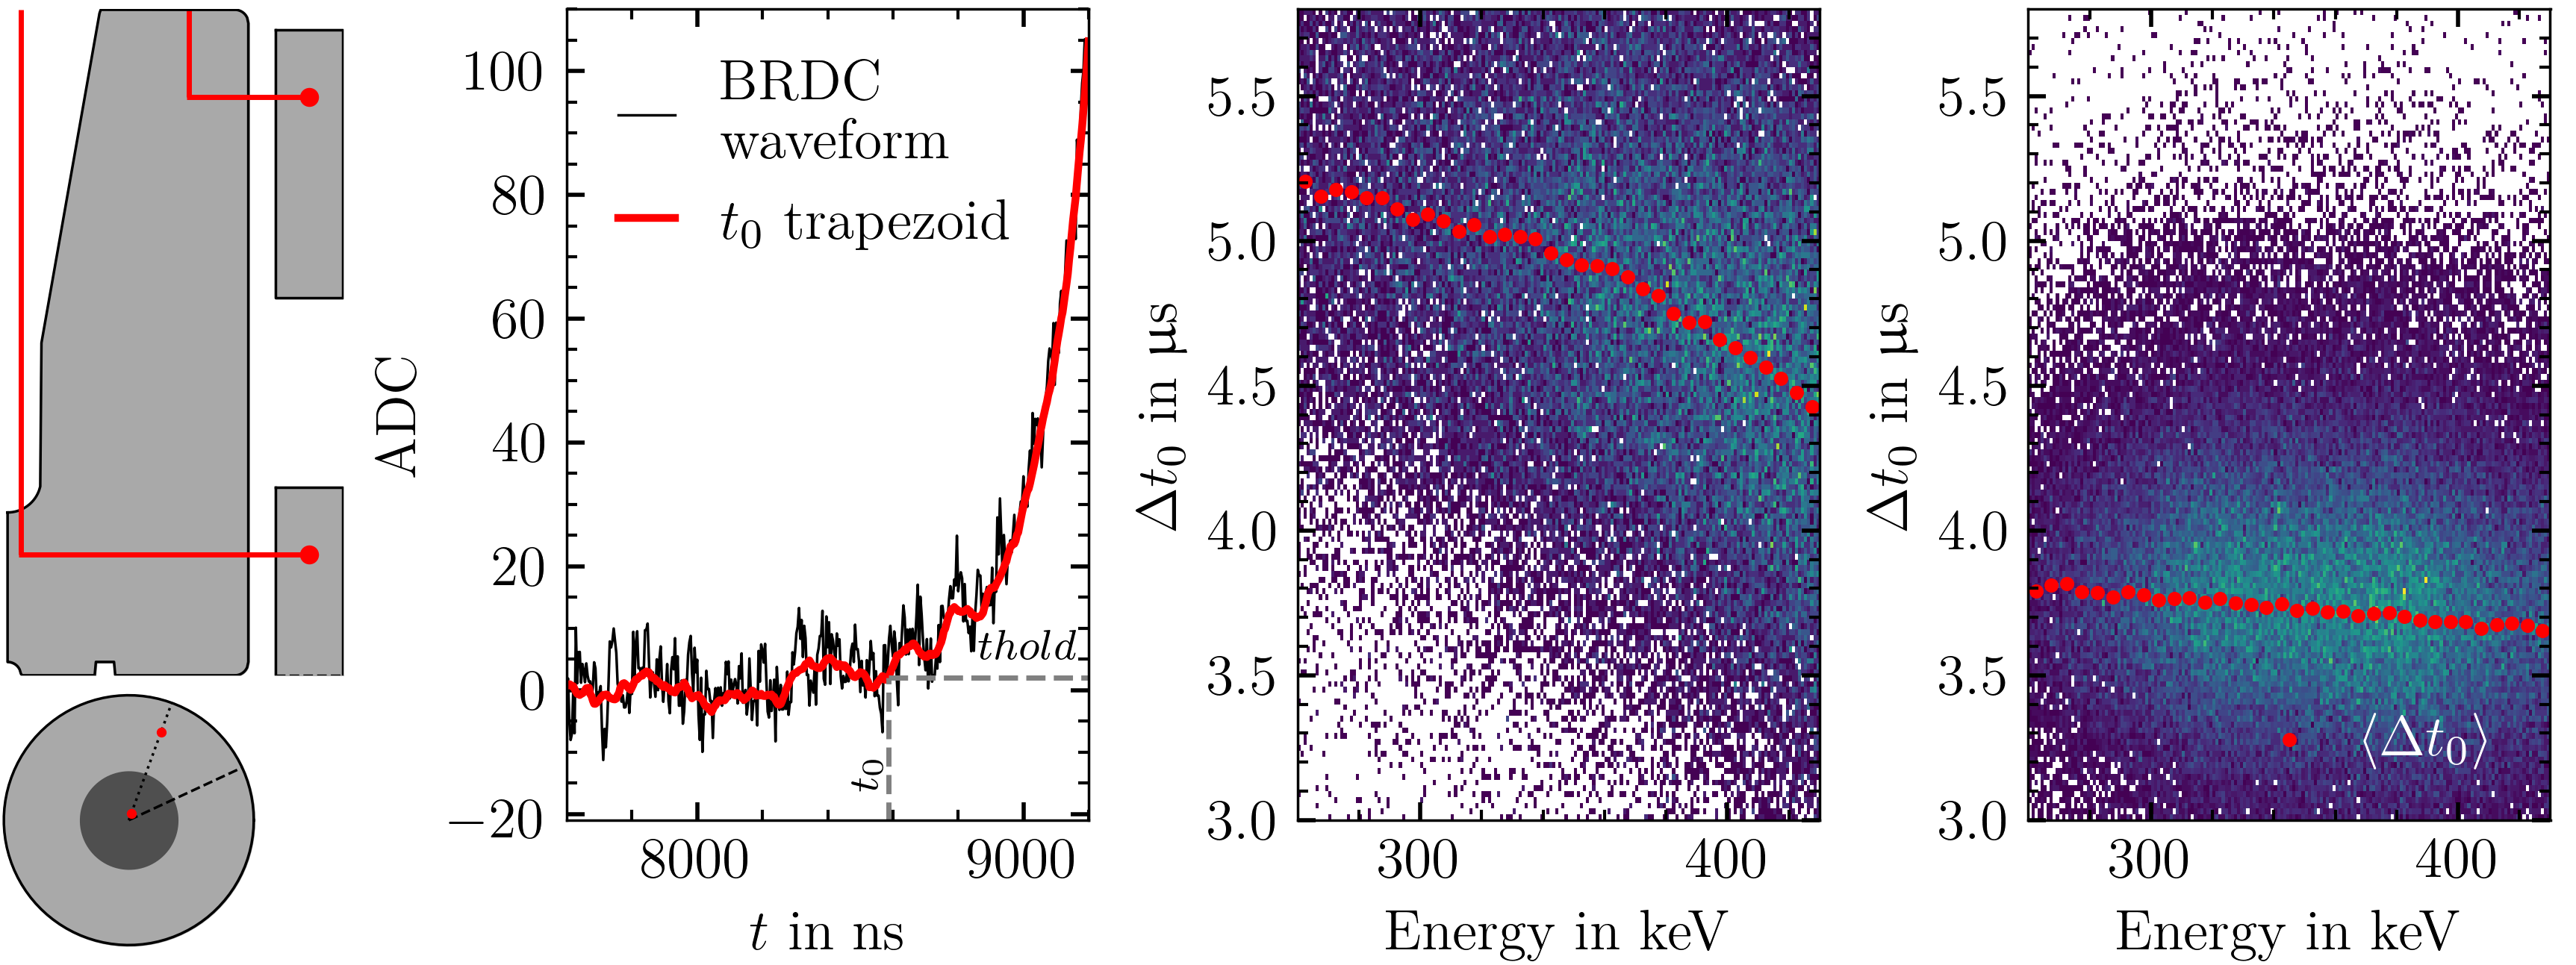
\includegraphics[width=6in]{figs/param/t0_bias.png}
    \caption{$t_0$ -- calculated as shown by the leftmost data panel -- is used to construct $\Delta t_0$ for each event for two distinct measurements. The first, represented in the pictogram with the camera position at the top of the detector corresponds to the middle data panel, while the bottom camera position corresponds to the rightmost panel. A total of 1.4e5 and 1.8e5 events pass the fully contained cut described in the text respectively. The mean, $\left< \Delta t_0 \right>$, is calculated from 5\,keV wide energy bins, and plotted in red. The color in the 2D histograms is shown in linear scale.}
    \label{fig:t0_bias}
\end{figure}

Since $t_0$ is determined from a threshold crossing, lower energies are biased towards later $t_0$'s. To calculate the magnitude of this effect a reference event time is needed. For coincident Compton events, the trigger time of the camera can be used for this purpose. The difference between event onsets at a given ICPC energy, $E$, in the ICPC and camera is given by $\Delta t_0$:
\begin{equation}
	\Delta t_0(E) = (t_\text{IC}(E) + t_0(E)) - t_\text{CAM}(662\,\text{keV} - E)~,
	\label{eq:t0_bias}
\end{equation}
where $t_\text{IC}$ and $t_\text{CAM}$ are the detector and camera DAQ trigger times respectively. Note that only events that were fully contained in both detectors -- $\left|E + E_\text{CAM} - 662\,\text{keV}\right| \leq 8\,\text{keV}$ -- are used. Ideally, $t_0$ would also be calculated for the camera. However, these waveforms are not saved, and only the camera DAQ trigger time is available. Moreover, by the nature of coincident Compton data, $t_\text{CAM}$ is not a constant reference: it has the opposite timing bias of the ICPC. $t_0(E)$ bias decreases monotonically with $E$, while $t_\text{CAM}(662\,\text{keV} - E)$ bias increases with $E$. Thus, a negative slope is always expected for $\Delta t_0(E)$. This can be observed in the behavior of $\left< \Delta t_0 \right>$ in the two rightmost panels of Fig.~\ref{fig:t0_bias}. Here, $\Delta t_0$ is plotted against energy for all fully contained coincident events with constant \CsS{} source and camera position.  Note that if no camera timing bias would exist, or if only monoenergetic camera events were used, $\Delta t_0(E)$ would exhibit asymptotic behavior as exemplified in Ref.~\cite{mjd_charge_trapping} with coincident \ThS{} data.

It is not possible to disentangle the ICPC from the camera timing bias from a single measurement. Nevertheless, some inroads can be achieved by exploiting the event position sensing capabilities of the Compton scanner. Events close to the point-contact of the ICPC are expected to have very little timing bias due to their very steep rise. By placing the \CsS{} over the point-contact and aligning the camera with this region in the ICPC, a reference $\left< \Delta t_0 \right>$ is constructed, to which the $\left< \Delta t_0 \right>$ of other regions of the detector can be compared. In particular, the upper arms of the detector can be targeted as shown in the pictogram of Fig.~\ref{fig:t0_bias}. Note that the depicted energy range of 260\,keV - 430\,keV, restricts the Compton angle to roughly $(90\pm30)^\circ$, constraining the targeted volume.

It is safe to assume that the camera timing bias remains constant over these two measurements, since the same energy range is used, and the camera is fully illuminated in both cases. Thus, the camera bias (and the constant offset between the DAQ times of the ICPC and camera) can be ``subtracted off'' in the following operation: $\left< \Delta t_0 \right>_\text{arm} - \left< \Delta t_0 \right>_\text{p-contact}$. The result suggests that the true onset of events in the upper arms of the detector is 0.8\,$\upmu$s-1.4\,$\upmu$s earlier than the computed $t_0$. These extrema correspond to ICPC energies of 430\,keV and 260\,keV respectively. The very low weighing potential in the arms of the detector is responsible for this effect.

Although expected, this finding has profound implications (in the stated energy range) for the calculation of drift time and to a lesser extent energy, which both depend on this variable. 

\section{Energy Estimation}\label{sec:energy}

The raw energy was estimated from a fixed-time-pickoff of a 4.5\,$\upmu$s-3.5\,$\upmu$s-4.5\,$\upmu$s trapezoidal filtered waveform. The flat time was set to almost twice the maximum drift time, allowing for the entire drift and the overshoot and successive settling from the electronics response to fit in this window. On the other hand, the rise and fall time were maximized within the constraints of the length of the recorded pulses. As opposed to the conventional method of using the maximum of the resulting trapezoid, where the statistics of the noise is governed by a series of samples, the use of one sample (the fixed-time-pickoff sample) reduces the bias to higher energies~\cite{mjd_charge_trapping}. This sample, denoted here as $t_\text{pick} = t_0 + (4.5+3.5-0.4)\,\upmu$s, was constructed as follows. The rise and flat time of the trapezoidal filter are added to $t_0$. An additional offset, determined empirically, ensures that $t_\text{pick}$ lies before the falling edge of the trapezoid. The procedure for raw energy estimation is illustrated in Fig.~\ref{fig:Cs_energy_calculation}.

The fixed-time-pickoff results in an ADC value which is converted into energy. The energy calibration parameters (a multiplicative constant and offset) are determined by fitting the peaks in the raw spectrum and paring them with tabulated peak energies. For convenience the spectra shown here (and previously) depict the calibrated raw energy. The calibrated energy spectrum in the vicinity of the 662\,keV \CsS{} energy peak is shown for resting baseline and soft pileup events in Compton data in Fig.~\ref{fig:Cs_energy_calculation}. Even though a coincidence filter is applied in Compton data, sufficient accidental coincidences with full energy peak events occur to monitor the ICPC's energy resolution during Compton scans in-situ. 
\begin{figure}[htb]
    \centering
    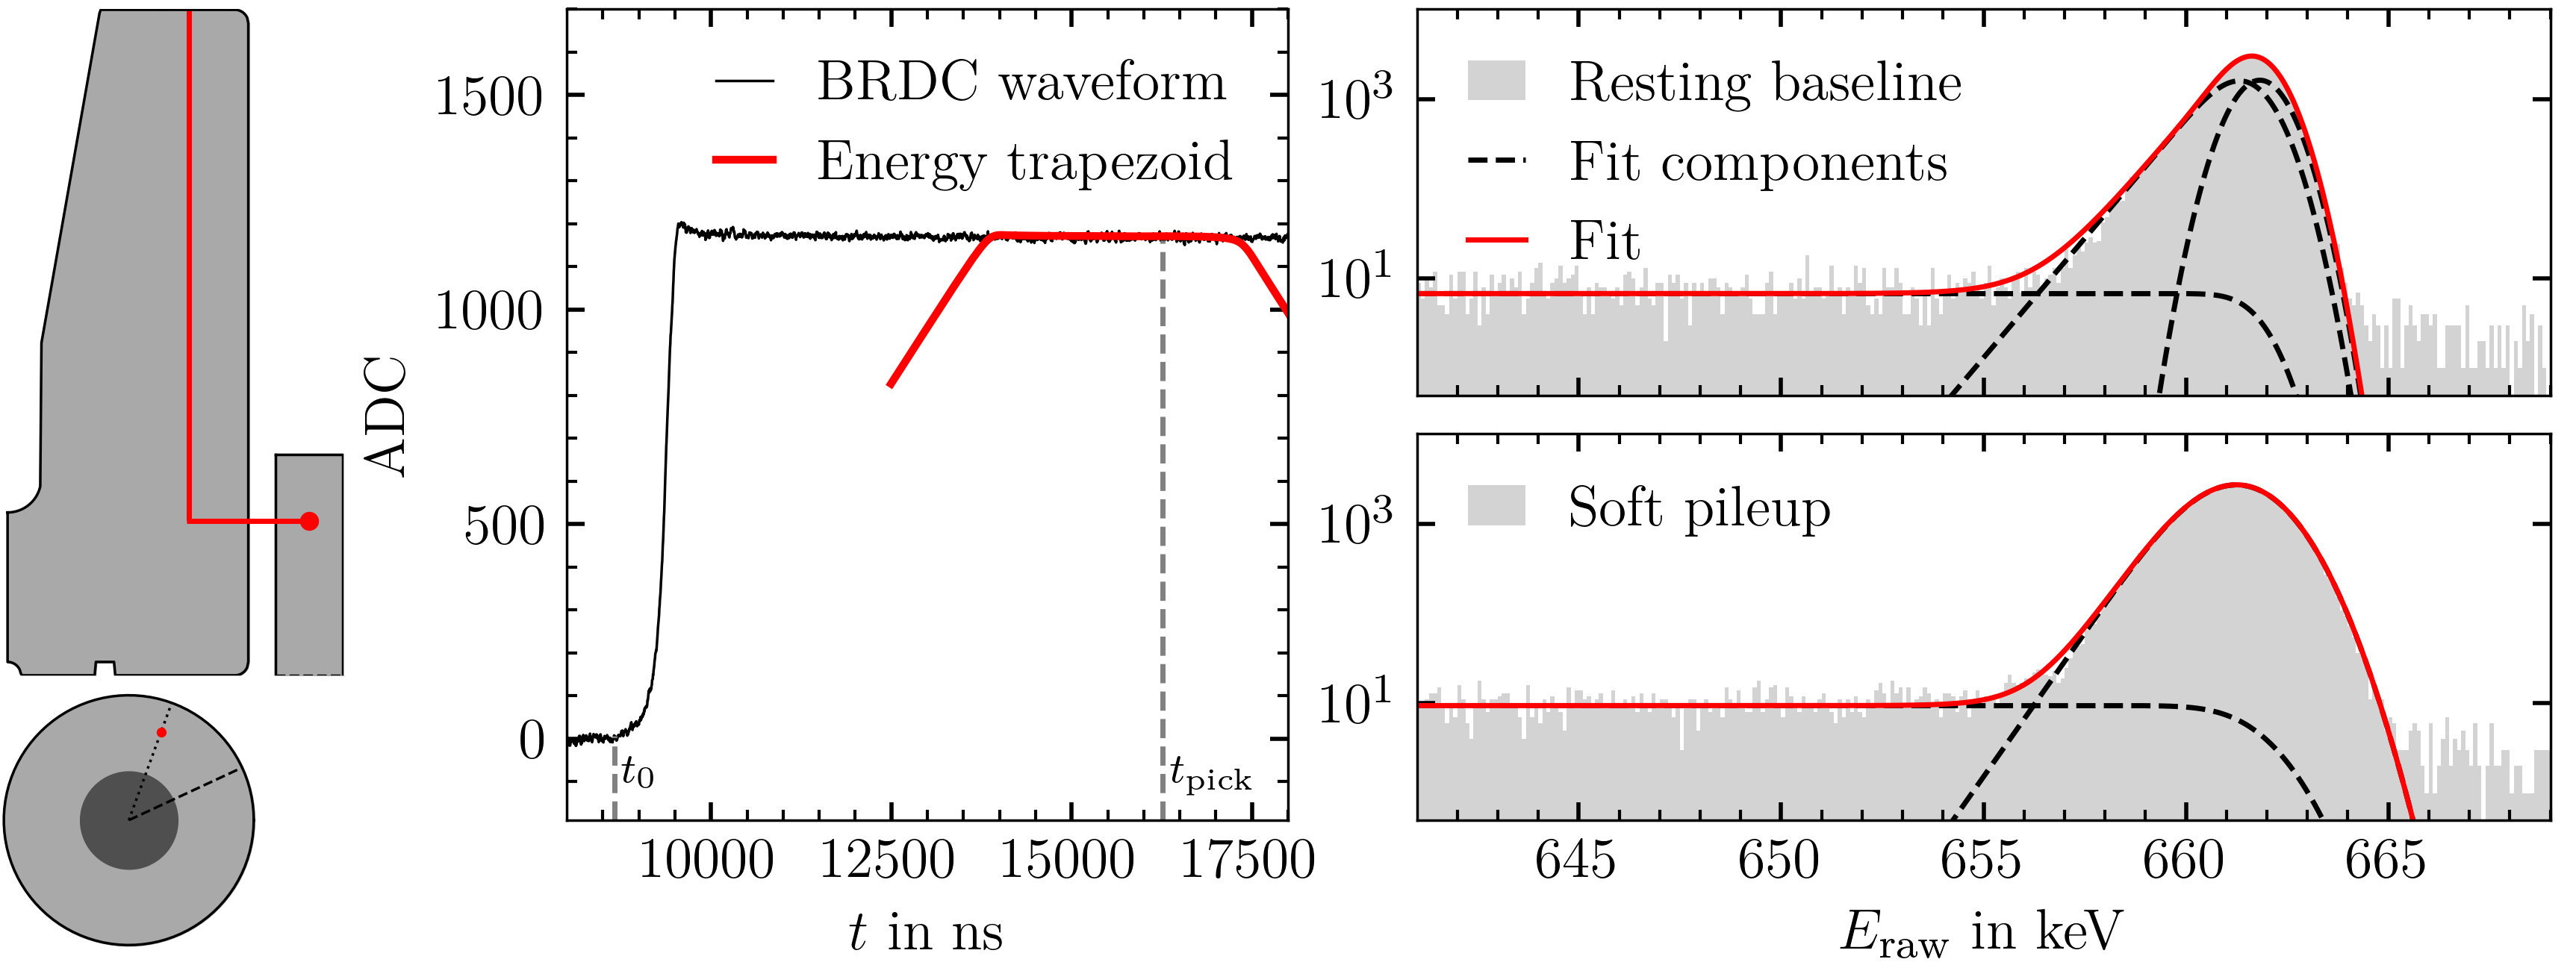
\includegraphics[width=6in]{figs/param/Cs_energy_calculation.png}
    \caption{The energy is calculated as the leftmost data panel illustrates to generate the spectra in the right. Note that the recorded baseline is too short to generate the full rise of the trapezoid. Nevertheless, $t_\text{pick}$, is situated well within the region of the trapezoid which can be calculated.}
    \label{fig:Cs_energy_calculation}
\end{figure}

All energy peaks are fit to a response function which captures the statistical effects of charge collection. An exponentially modified Gaussian low-energy tail is added to model incomplete charge collection due to charge trapping. It also includes contributions from residual soft pileup. The ICPC's response function $R(E)$ to a monoenergetic line $\mu$ follows. 
\begin{equation}
	R(E) = \frac{1-f}{\sqrt{2\pi\sigma^2}}e^{-\frac{(E-\mu)^2}{2\sigma^2}} + \frac{f}{2\gamma}e^{\left(\frac{\sigma^2}{2\gamma^2}+\frac{E-\mu}{\gamma}\right)}\text{erfc}\left(\frac{\sigma}{\sqrt{2}\gamma} + \frac{E-\mu}{\sqrt{2}\sigma}\right)
	\label{eq:energy_peak_fit}
\end{equation}
``where $\sigma$ represents the smearing due primarily due to electronics noise and charge collection statistics, $\gamma$ is the decay constant of the low-energy tail, and $f$ is the fraction of the peak shape contained in the low-energy tail''~\cite{MAJORANA2019}. The background is modeled as a complimentary error function plus a second order polynomial. For soft pileup events, a best fit parameter of $f \approx 1$ was found for all fit peaks. The FWHM extracted from the response function fits to the resting baseline and soft pileup spectra is 1.74\,keV and 2.66\,keV respectively at 662\,keV. 

Although there is a significant energy resolution degradation for soft pileup events, a FWHM of 2.66\,keV at 662\,keV remains well below the energy resolution of the camera. The desired spatial resolution of $\pm1$ in $z$ can be achieved by using the energy registered by the camera alone (using $E = 662\,\text{keV} - E_\text{CAM}$ for the ICPC). However, ICPC energy resolutions below that of the camera results in improved spatial resolution. Thus, although sufficient, the soft-pileup-event energy resolution is corrected to push its value closer to that of resting baseline events. 

\section{Soft Pileup Energy Corrections and Energy Calibration}\label{sec:ecorrcal}

As opposed to resting baseline events a correlation was observed between the slope of the corrected waveforms and the energy in soft pileup events. Any negative slope residual slope after MRDC correction shifts the energy towards lower values, while positive slopes have the opposite effect. This correlation can be observed in the leftmost data panel of Fig.~\ref{fig:soft_pileup_e_corr}.
\begin{figure}[htb]
    \centering
    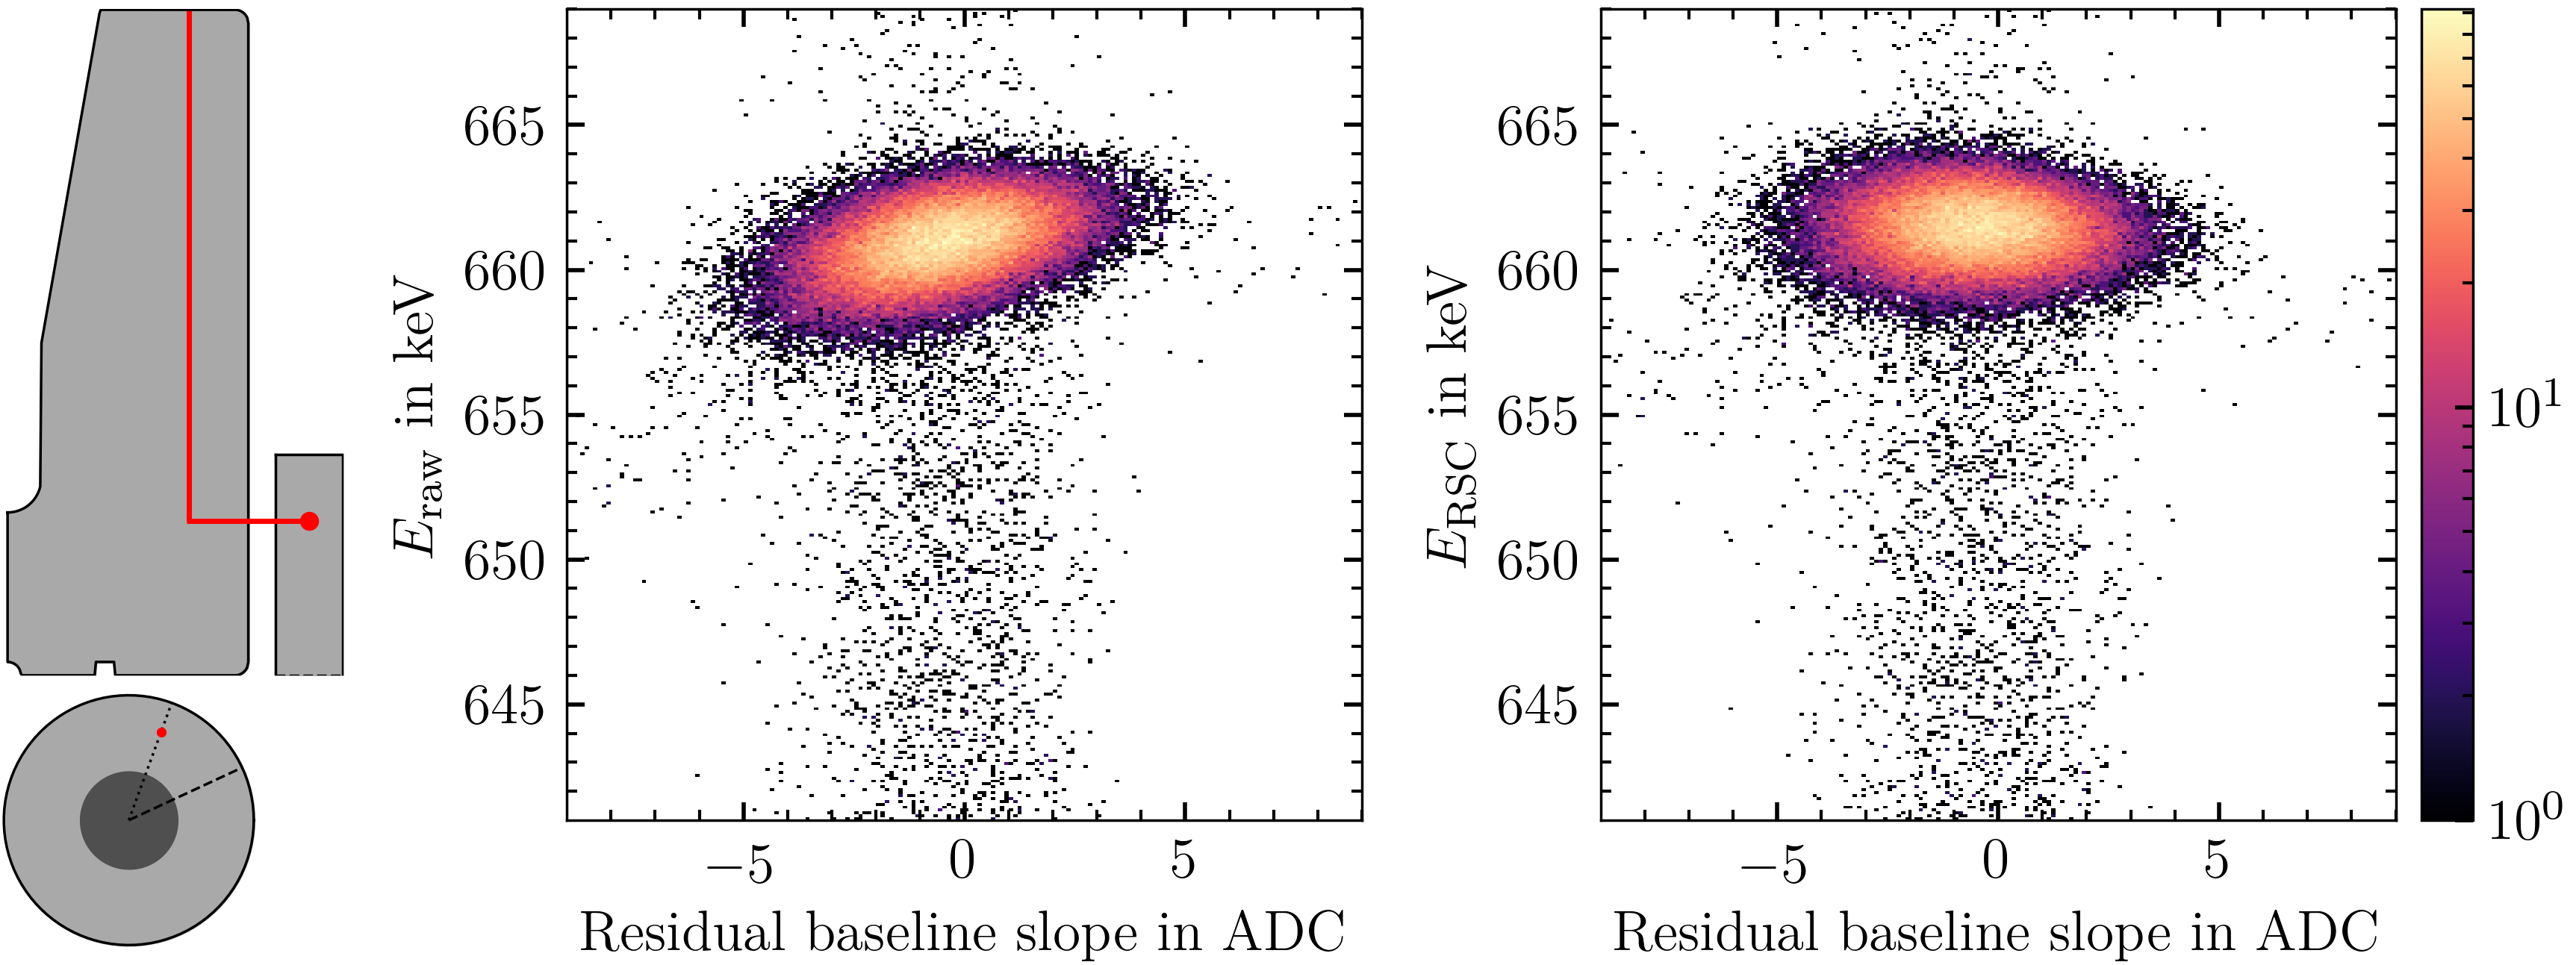
\includegraphics[width=6in]{figs/param/soft_pileup_e_corr.png}
    \caption{The raw and RS corrected slope-energy correlation is shown on the left and right respectively for accidental coincidences between full energy 662\,keV gamma events in the ICPC and camera.}
    \label{fig:soft_pileup_e_corr}
\end{figure}

To correct for this effect a linear residual slope correction to the energy ($E_\text{RSC}$) is applied to soft pileup events as follows.
\begin{equation}
	E_\text{RSC} = E_\text{raw} - r_{rs} \times B_{rs}
\end{equation}
where $B_{rs}$ is the baseline slope of the MRDC waveform (also referred to as residual baseline slope), and $r_{rs}$ is the residual slope (RS) correction constant. $r_{rs}$ is determined by successive application of the correction and fits to the resulting energy over a range of values. The constant which minimizes the fit FWHM is adopted. Applying the correction with $r_{rs} = 0.60$ to the data shown in Fig.~\ref{fig:soft_pileup_e_corr}, a FWHM of 2.46\,keV is achieved (down from 2.66\,keV). The optimal RS correction constant value varies slightly depending on the location of the source, therefore, the value quoted above is determined from the same flood \ThS{} measurement used to determine the energy calibration parameters.

As introduced in Sec.~\ref{sec:pileup}, the data from this flood measurement is split into two data streams: soft pileup and resting baseline events. The raw energy is calculated for each and calibrated with the 277\,keV ($^{208}$Tl), 300\,keV ($^{212}$Pb), 583\,keV ($^{208}$Tl), 727\,keV ($^{212}$Bi), 861\,keV ($^{208}$Tl), and 2615\,keV ($^{208}$Tl) full energy gamma peaks. To perform the calibration the peaks in both data streams are fit using their respective response functions defined in the previous section. For resting baseline events a simultaneous fit of the peaks is performed. The fit determines a common low-energy tail fraction of $f = 0.48$.
\begin{figure}[htb]
    \centering
    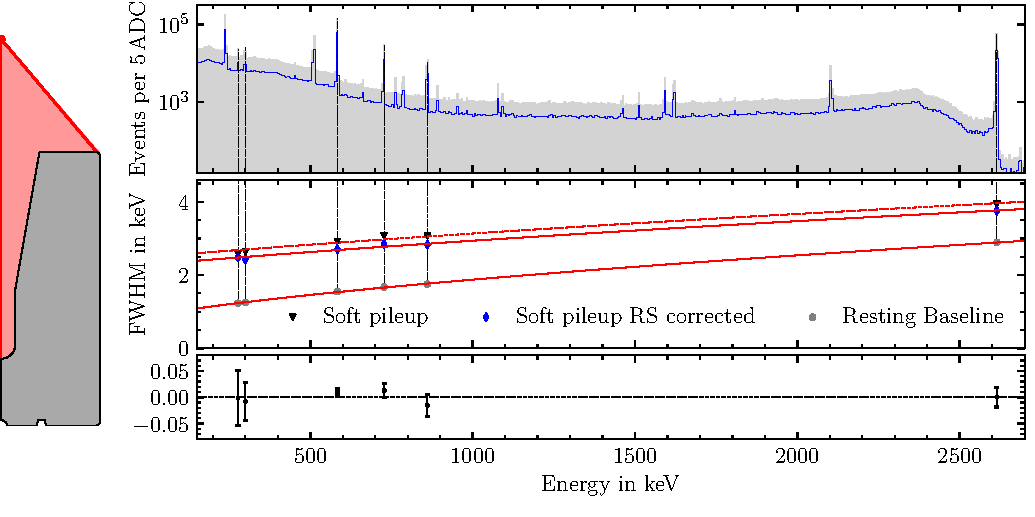
\includegraphics[width=6in]{figs/param/fwhm_peaks.pdf}
    \caption{The calibrated raw energy (gray) and calibrated RS corrected energy (blue) spectra are shown in the top data panel for resting baseline events and soft-pileup events respectively. Note that different calibration parameters are used for each data set, such that all points align at the tabulated calibration peak energies listed in the text. The FWHM extracted from each fit peak is shown in the panel below, including a fit in red to Eq.~\ref{eq:energy_fwhm}. The calibrated raw energy for soft-pileup events is included for reference, with a fit in dashed red. In the bottom panel the residual of the fit is shown along with the FWHM error (numerically extracted from the peak fits) for resting baseline events.}
    \label{fig:fwhm_peaks}
\end{figure}

The RS corrected soft-pileup event energy is calibrated using the same peak fit response function as its uncorrected counterpart. In summary, three distinct calibration constants are computed: for resting baseline events, soft pileup events and RS corrected soft pileup events. The FWHM is determined for each peak fit numerically. The results are summarized in Fig.~\ref{fig:fwhm_peaks} where the peak FWHM's are fit to Eq.~\ref{eq:energy_resolution}, repeated here in terms of FWHM for convenience. 
\begin{equation}
	\text{FWHM}(E) = \sqrt{\Gamma_n^2 + \Gamma_F^2E + \Gamma_q^2E^2}
	\label{eq:energy_fwhm}
\end{equation}
The floating terms $\Gamma_n$, $\Gamma_F$ and $\Gamma_q$ account for noise, charge collection statistics and incomplete charge collection. For soft-pileup events, $\Gamma_n$ includes a dominant contribution from the imperfect decay correction. This effect completely obscures charge trapping effects and thus $\Gamma_q$ is set to zero for soft pileup fits.  

A modest improvement is achieved by the RS correction across the entire spectrum, effectively reducing the value of $\Gamma_n^2$ by 16\%. Unless otherwise stated, the energies used in all analysis from this point forward are the calibrated raw energy and calibrated RS corrected energy for resting baseline events and soft-pileup events respectively, simply denoted as $E$. 

The same analysis was repeated on data taken with the \ThS{} source positioned on the side of the detector, 9\,cm away and approximately level with the p$^+$ contact. In this configuration, the source illuminates the bottom of the detector, where shorter drift paths prevail, more effectively. Since such events are less subject to charge trapping, an improved energy resolution is expected. The energy resolution for resting baseline and RS corrected soft pileup events in the top and side \ThS{} measurements are summarized in Tab.~\ref{tab:fwhm_Tl}.
\begin{table}[tbph]
    \centering
    \caption{A summary of \ThS{} calibration energy resolution. The low energy tail fraction is obtained from a simultaneous fit to the calibration peaks listed in the text. For the side measurement the two lowest peaks do not appear in the spectrum and are not included in the fit. Note that $f$ is set to 1 for soft pileup events.}
	\vspace{12pt}
	\begin{tabularx}{1\textwidth}{>{\tr}X >{\tr}X >{\tr}X}
		\hline \noalign{\vskip 1ex}
		\quad Population & Low-energy tail fraction $f$ & 2615\,keV $^{208}$Tl FWHM in keV\\[1ex]
		\hline \noalign{\vskip 1ex}
		\multicolumn{3}{l}{Top \ThS{} source position} \\[1ex]
		\quad Resting baseline & 0.48 & 2.91\\
		\quad RSC Soft pileup & -- & 3.76\\[1ex]
		\multicolumn{3}{l}{Side \ThS{} source position} \\[1ex]
		\quad Resting baseline & 0.55 & 2.56\\
		\quad RSC Soft pileup  & -- & 3.26\\[1ex]
		\hline
	\end{tabularx}
	\label{tab:fwhm_Tl}
\end{table}

\section{Drift Time Calculation}
The drift time, or the time from $t_0$ to say $t_{99}$ (time at which 99\% of the total induced charge is reached), requires the calculation of two threshold crossings. As seen in Sec.~\ref{sec:t0}, threshold crossings are subject to bias and noise. It is thus beneficial to avoid the calculation of $t_{99}$. In Sec.~\ref{sec:charge_trapping} the integral of uncollected charge, $D$, was introduced. This variable can be used as a proxy for drift time, although its real units are time $\times$ charge. Fig.~\ref{fig:dt_calculation} shows the procedure dictated by Eq.~\ref{eq:uncollected_charge}: $D$ is equal to the area in gray minus the area in red divided by 3\,$\upmu$s, resulting in an ADC value. Shorter drift times thus result in smaller values of $D$.
\begin{figure}[htb]
    \centering
    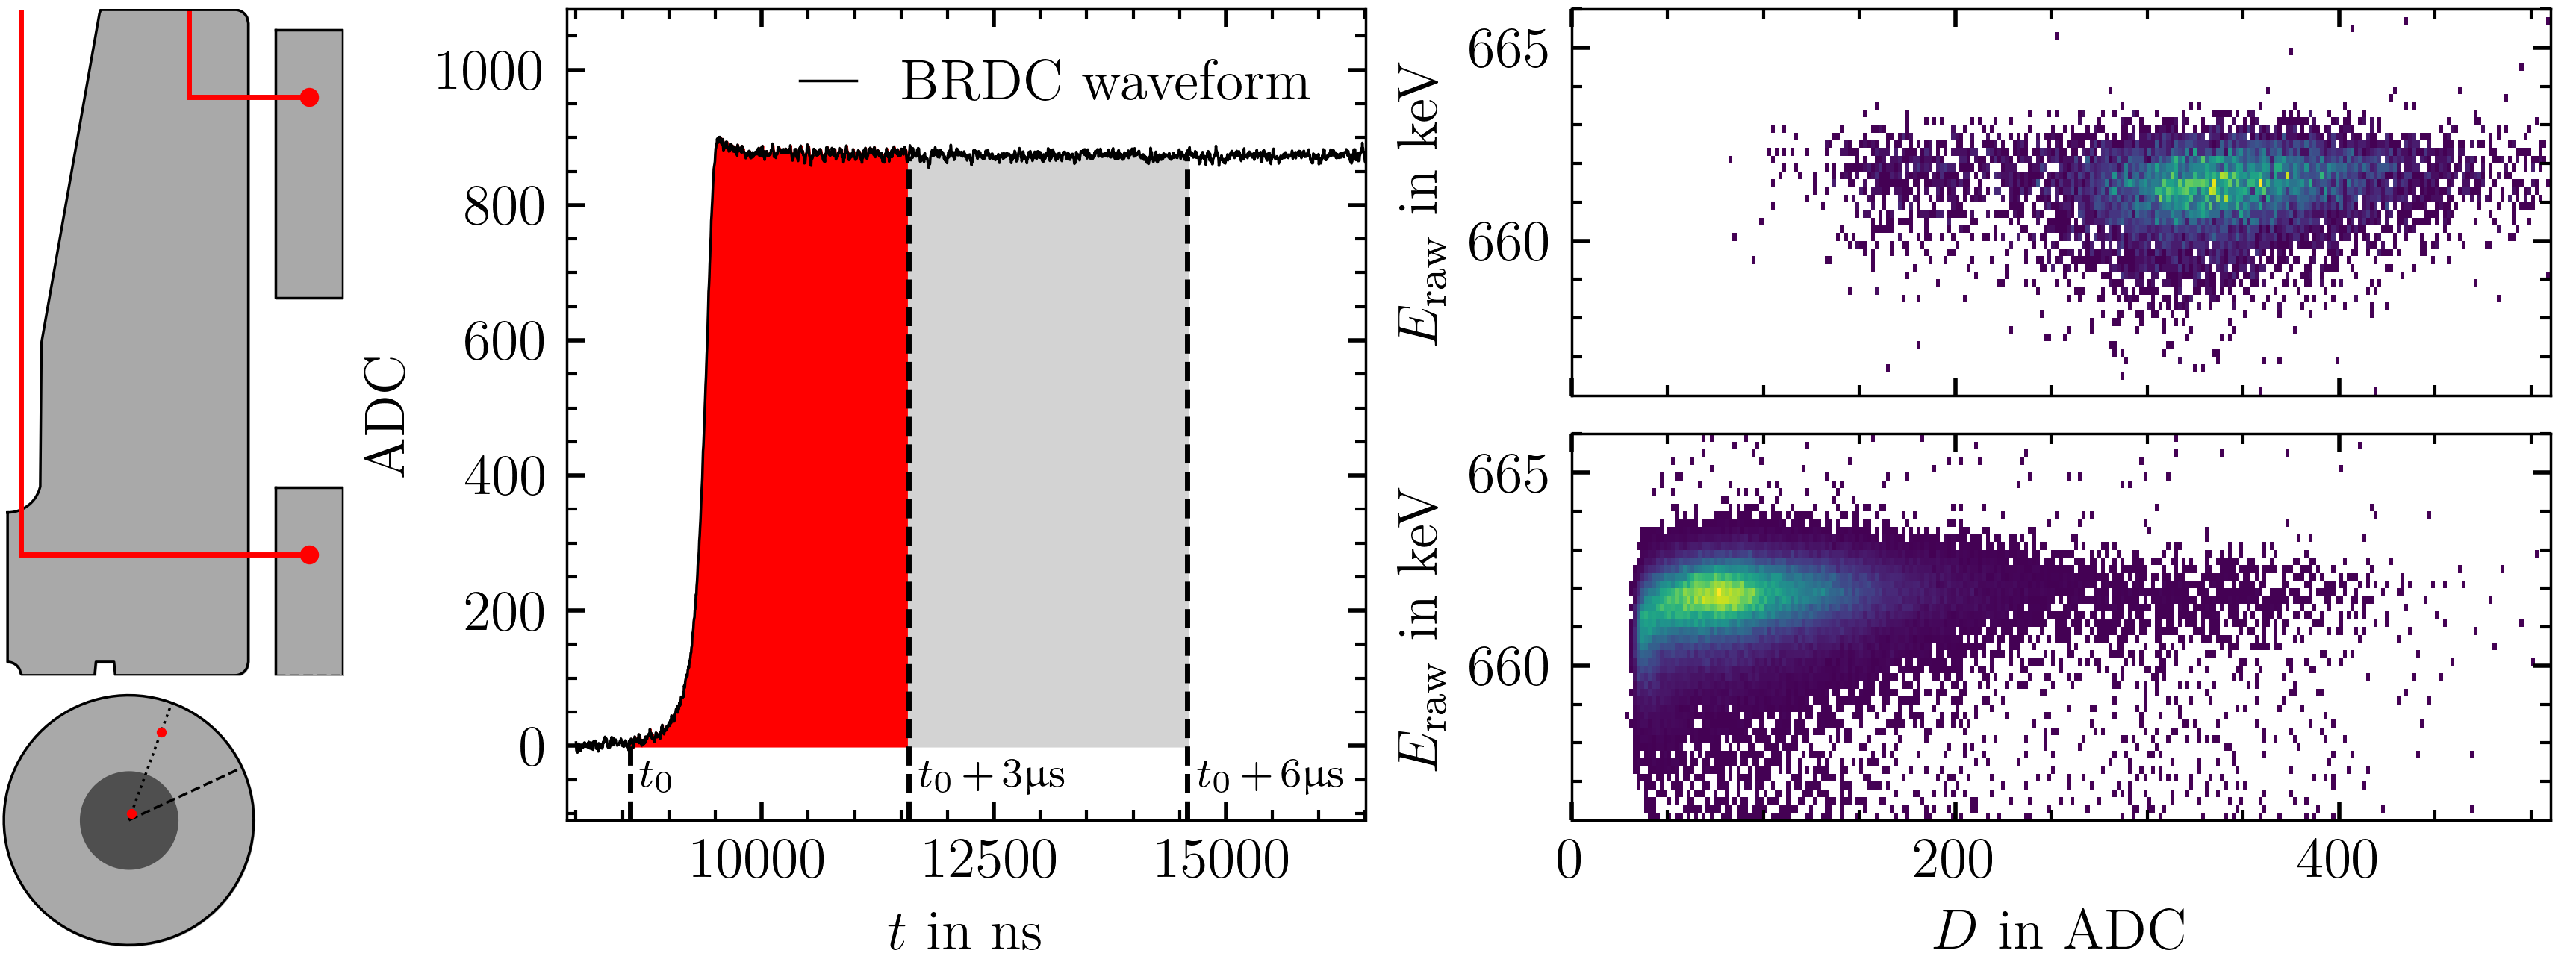
\includegraphics[width=6in]{figs/param/dt_calculation.png}
    \caption{The integral of uncollected charge is calculated as described in the text and exemplified by the leftmost data panel. On the right, the $D$ is shown for resting baseline accidental 662\,keV coincidences close to the point-contact ($r = 1$\,mm, bottom panel) and further away ($r = 27$\,mm, top panel).}
    \label{fig:dt_calculation}
\end{figure}

Fig.~\ref{fig:dt_calculation} also shows the $D$ distribution for the same data sets used in Sec.~\ref{sec:t0}. As expected much shorter drift times are obtained when the source is over the point-contact of the detector. As described in Sec.~\ref{sec:charge_trapping} charge clouds degrade exponentially with drift time. It immediately follows that the energy resolution improves as drift time decreases. This is seen in data, with a resting baseline energy resolution of 1.71\,keV and 1.56\,keV at 662\,keV for $r = 1$\,mm and $r = 27$\,mm respectively. Charge trapping can be mitigated by applying a $D$ dependent correction to the energy. 

\section{Charge Trapping Energy Correction}

The degree of charge trapping can be quantified to an extent by applying a charge trapping (CT) correction. A linear CT correction is applied to resting baseline events in a similar fashion to the RS correction for soft pileup events: a linear term, this time dependent on $D$, is added to the raw energy, and the coefficient is varied to minimize the energy resolution. The exact operation, based on Eq.~\ref{eq:energy_corr2}, follows:
\begin{equation}
	E_\text{CTC} = E_\text{raw} + r_{ct} \times D_\text{CTC}
	\label{eq:ct_energy_corr}
\end{equation}
where $r_{ct}$ is the linear charge trapping coefficient and $D_\text{CTC} \equiv (D-0.3E_\text{raw})/1000$. Note that opposed to $B_{rs}$, $D$ is not centered around zero, therefore the distribution of D is shifted in $D_\text{CTC}$ such that the correction does not result in major shifts to the energy. This particular form of $D_\text{CTC}$ was adopted from Ref.~\cite{ornl_analysis}.
\begin{figure}[htb]
    \centering
    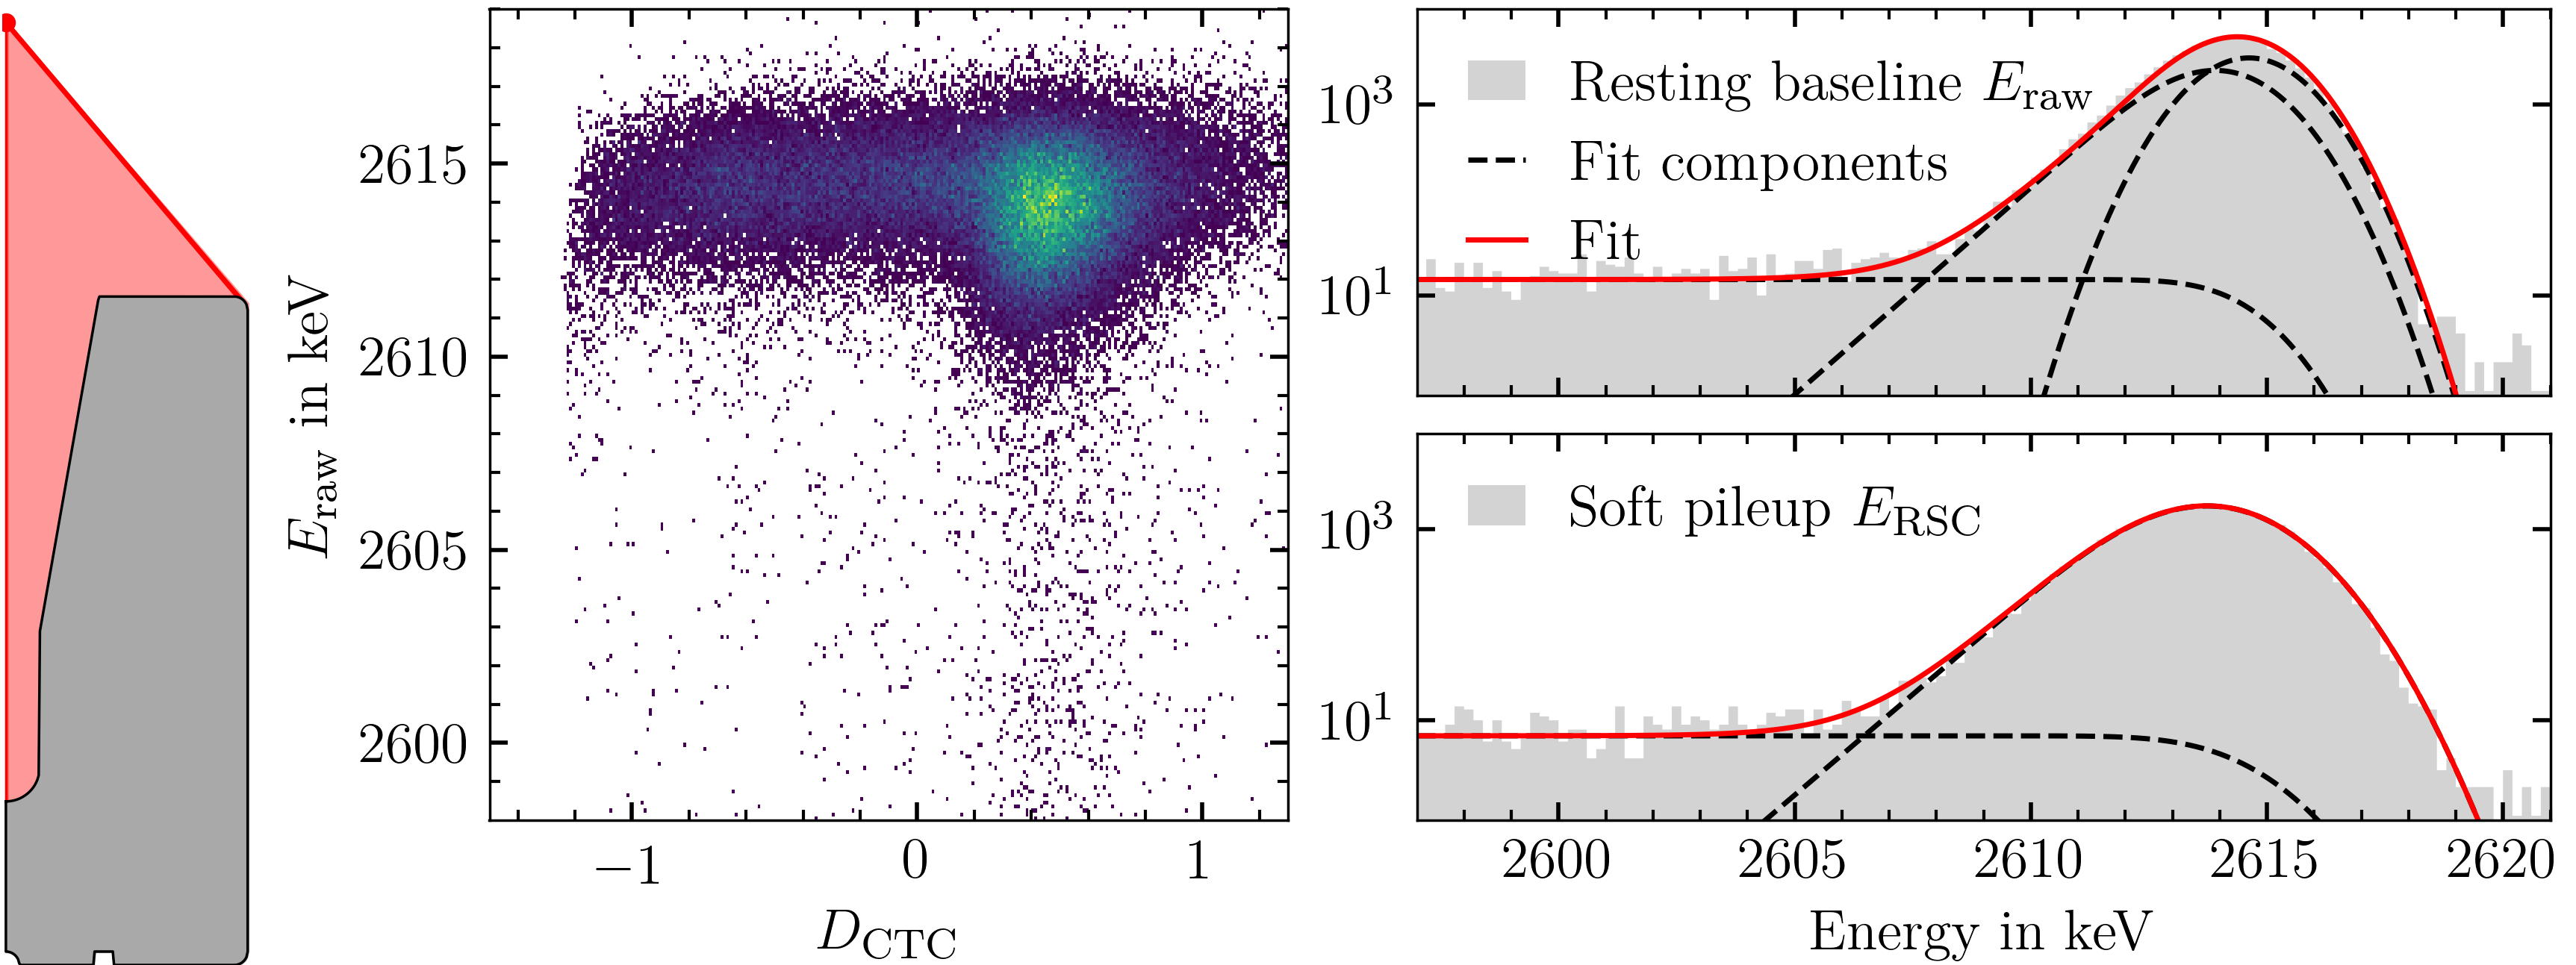
\includegraphics[width=6in]{figs/param/dt_e_corr.png}
    \caption{The $D_\text{CTC}$ distribution is shown on the left for the top \ThS{} measurement. The low weighting potential leads to a significant bias in the determination of $t_0$. Thus, similar values of $D_\text{CTC}$ are calculated for events along the arm of the detector, leading to events pilling up on the higher end of the distribution. Note that the same effect is seen when illuminating the detector from the side (where attenuation effects are lower) in the next figure. The peak shapes of the resting baseline and RS corrected soft pileup events are shown on the right.}
    \label{fig:dt_e_corr}
\end{figure}
\begin{figure}[htb]
    \centering
    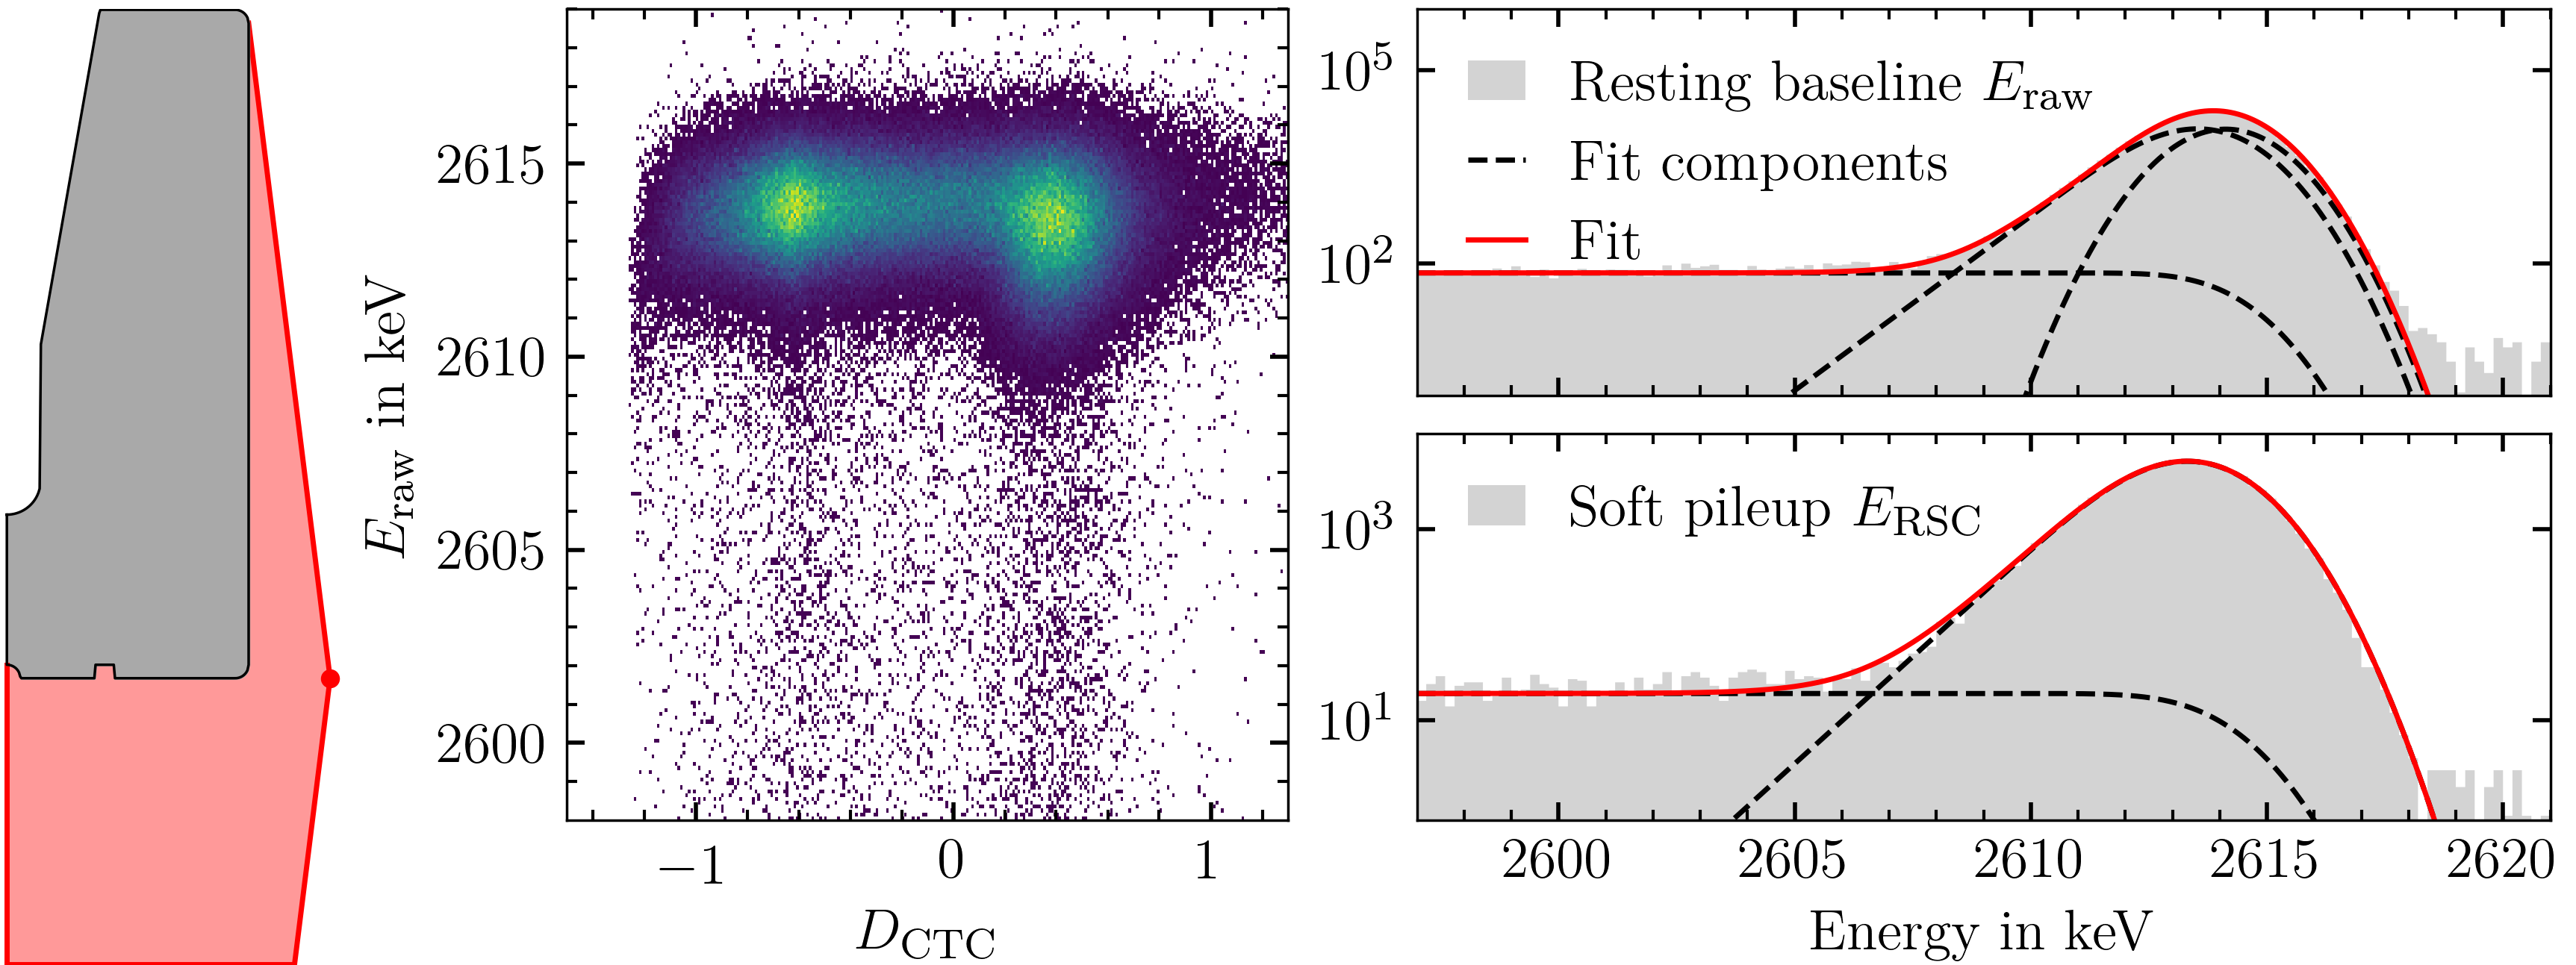
\includegraphics[width=6in]{figs/param/dt_e_corr_side.png}
    \caption{An equivalent analysis than in Fig.~\ref{fig:dt_e_corr} is shown for data taken with the \ThS{} source placed on the side on the detector.}
    \label{fig:dt_e_corr_side}
\end{figure}

The outlined procedure resulted in an optimal linear charge trapping coefficient of $r_{ct} = 0.1$ for the resting baseline data presented in Fig.~\ref{fig:dt_e_corr}. The positive value of $r_{ct}$ has the effect of adding charge back to the raw value, compensating for the slight negative slope seen in the $D_\text{CTC}$ distribution in leftmost data panel of the figure. However, the correction is too small to see any significant improvements in energy resolution or peak shape. The 2615\,keV peak shapes and fits for the top and side \ThS{} measurements are shown in Fig.~\ref{fig:dt_e_corr} and Fig.~\ref{fig:dt_e_corr_side} respectively, along with their $D_\text{CTC}$ distributions. 

\section{Multi-site Event Classifier}\label{sec:avse}

As introduced in Sec.~\ref{sec:workingprinciple}, multi-site events in the detector lead to misreconstructed event positions. The $\alpha$-reconstruction was shown to effectively reject against multi-site events in the n-type segmented PPC with which the Compton Scanner was commissioned with. However, gammas need to penetrate 2.5 times more Ge to reach the bottom of the ICPC detector than in the n-type PPC. This lead to a non-negligeble contamination of multi-site events passing the $\alpha$-validation when the \CsS{} was placed over areas with the highest surrounding amount of Ge (for example in the middle of the ICPC's arms). For this reason, a multi-site discriminator was employed to provide an additional layer of filtering against multi-site events. 

$A/E$ (introduced in Sec.~\ref{sec:bg_disc}) was considered as multi-site event classifier. Although effective at high energies, like at \Qbb{}, the $A/E$ distribution significantly broadens under 500\,keV, degrading its accuracy in the Compton continuum of \CsS{}. For this reason an alternative classifier -- $AvsE$ -- developed by the {\MJMit} Collaboration, is used. Instead of dividing $A$ (the maximum current amplitude) by $E$, the almost linear relation between $A$ and $E$ is fit to a second order polynomial and used to construct $AvsE$ as follows: 
\begin{equation}
	AvsE \equiv -(A_\text{cal} - p_0 - p_1E - p_2E^2)/j
	\label{eq:avse}
\end{equation}
where $A_\text{cal}$ is simply $A$ multiplied by the same constant used to calibrate $E$ and j is a positive constant determined by tuning $AvsE$ in such a way that events with $AvsE > -1$ are classified as single-site. The fit parameters, $p$, are determined by calculating the modes of $A_\text{cal}$ in small energy windows along the entire \ThS{} spectrum as shown in the bottom panel of Fig.~\ref{fig:avse_calculation}.
\begin{figure}[htb]
    \centering
    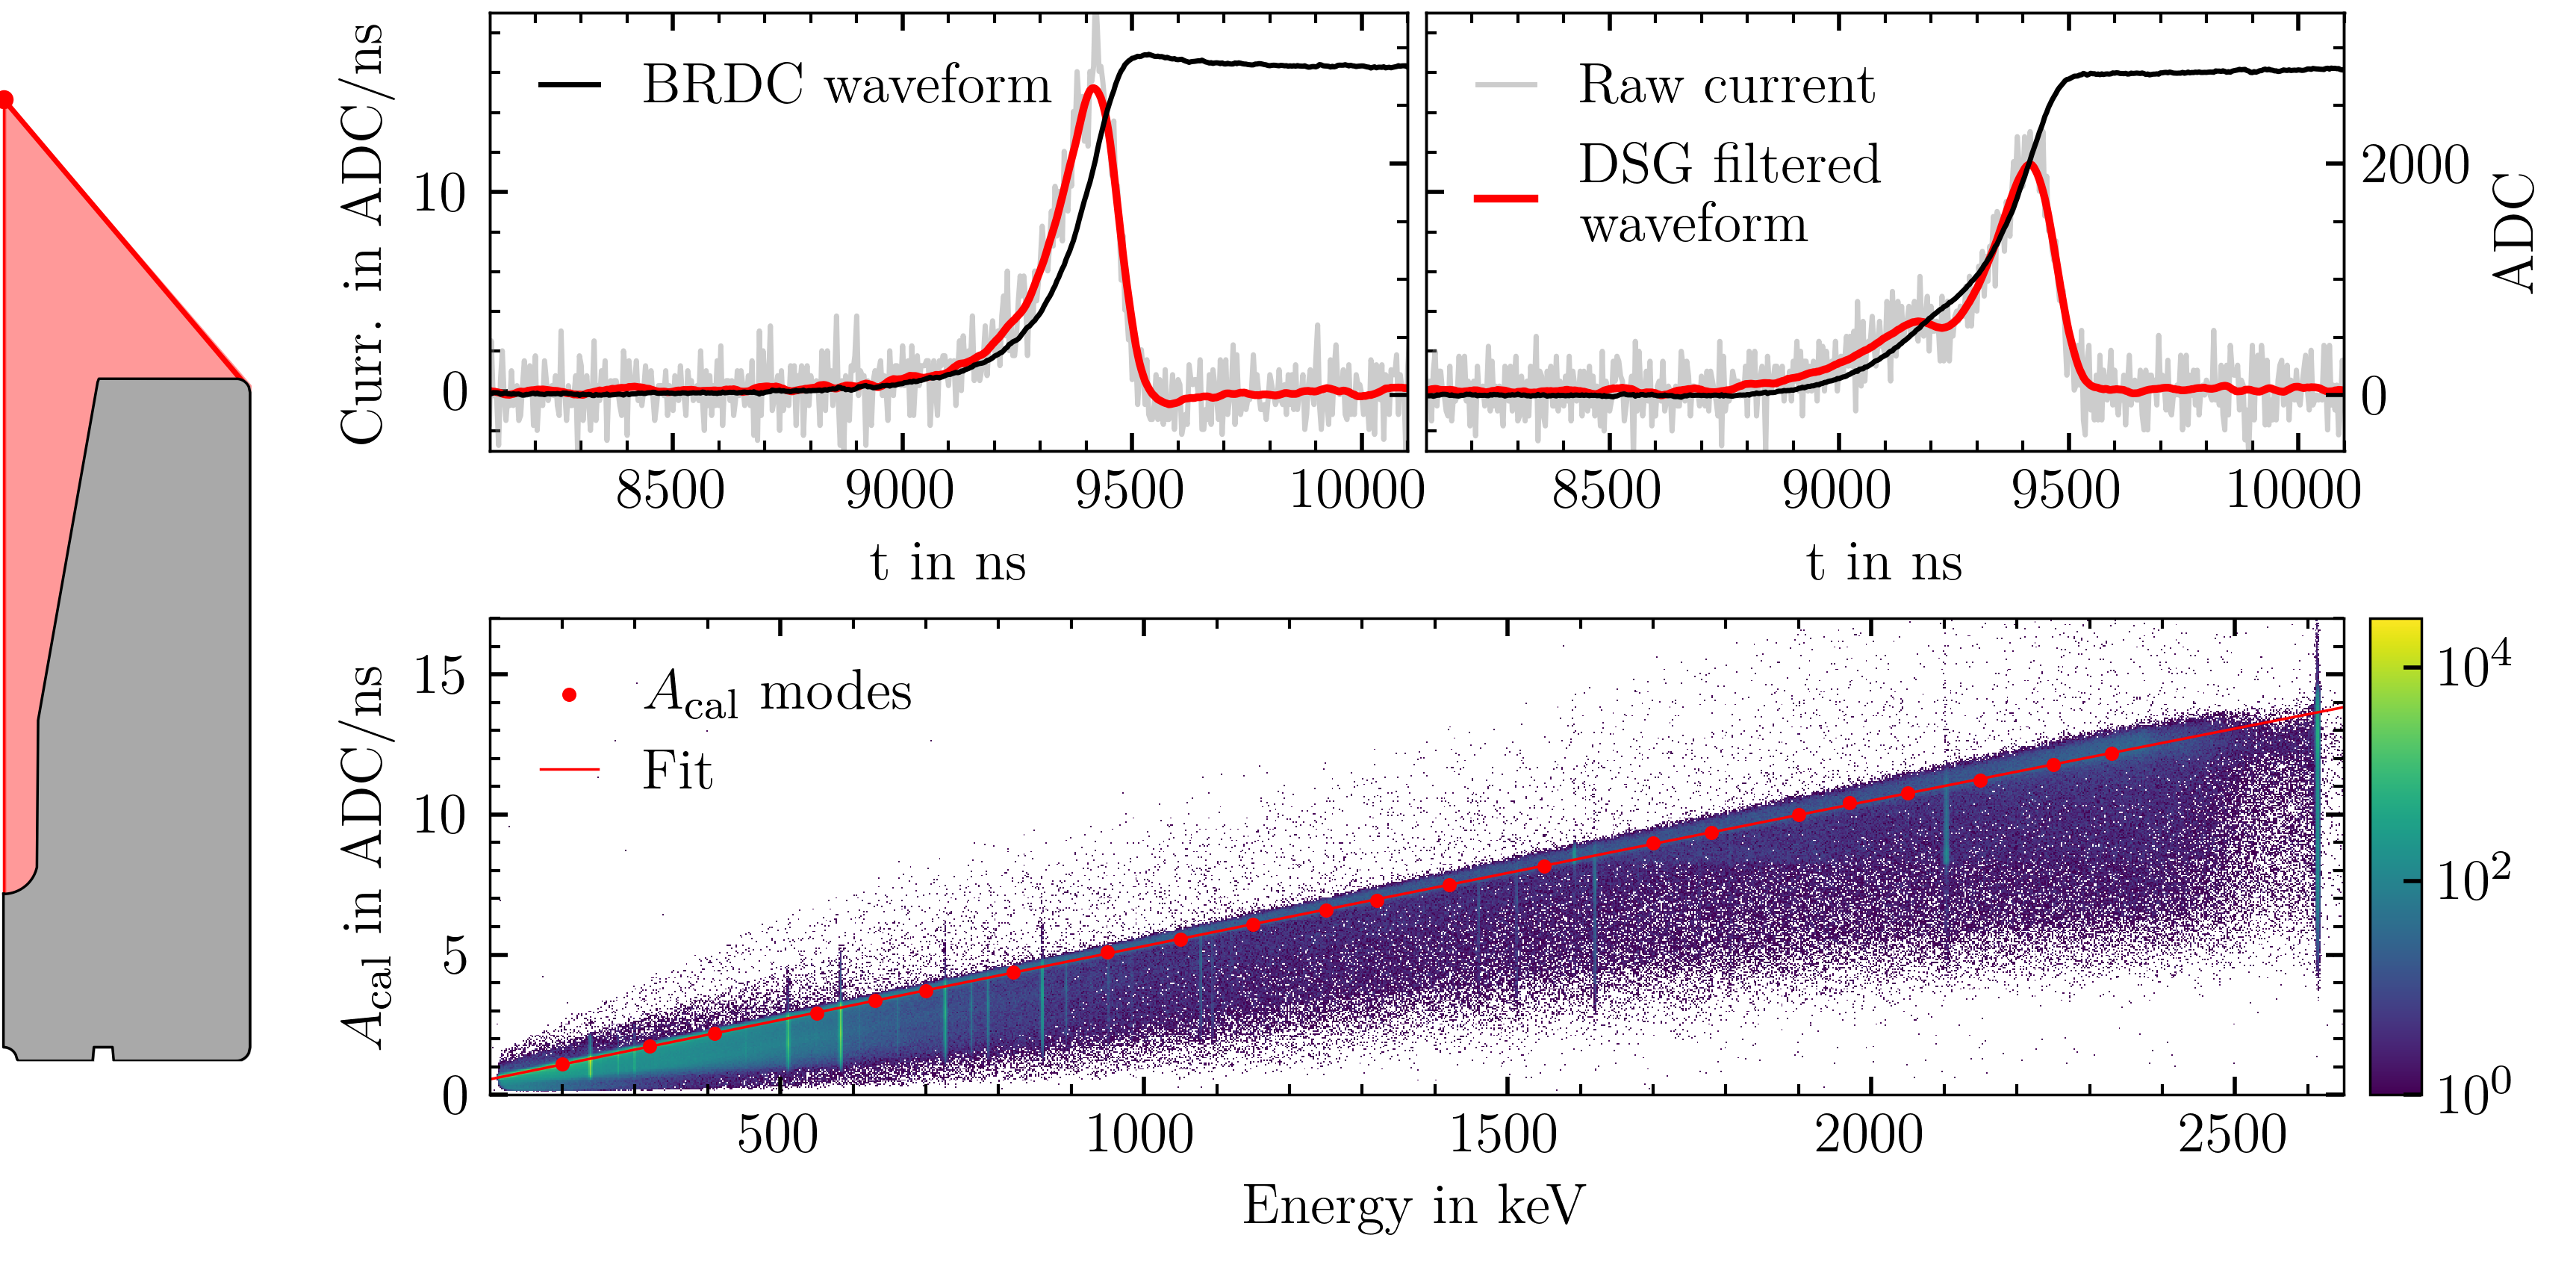
\includegraphics[width=6in]{figs/param/avse_calculation.png}
    \caption{A first degree differentiating Savitzky-Golay filter is applied to two DEP waveforms to obtain their respective $A$ values. The $A$ of the single-site event (top-left) is larger than that of a multi-site event of the same energy (top right). The raw current, that is the sample by sample derivative of the waveform, is shown in the background in gray for reference. $A_\text{cal}$ for resting baseline events are shown in relation to  $E$ in the bottom panel. The red points correspond to the $A_\text{cal}$ modes obtained in 10\,keV-wide evaluation windows centered at each point. The points are chosen as to not coincide with any peak in the spectrum and fit as described in the text.}
    \label{fig:avse_calculation}
\end{figure}

In Compton data, the $AvsE$ classifier was tuned with events reconstructed in the regions with the least surrounding Ge (in the outer edge or in the middle the detector). Reconstructed events passing $\alpha$-validation in these regions constitute a population of >90\%-pure single-site events. These results are outlined in Sec.~\ref{subsec:singlesitecompton}. However, Compton data provides a very small energy window over which $AvsE$ can be constructed. For this reason, $AvsE$ is constructed using the parameters calculated in this section, and tuned for Compton data with the aforementioned reconstructed events. In this section tuning is performed with the standard DEP and SEP events as reference populations of single- and multi-site events. More concisely, $AvsE$ is tuned to retain 90\% of DEP events in the analysis that follows. 
\begin{figure}[htb]
    \centering
    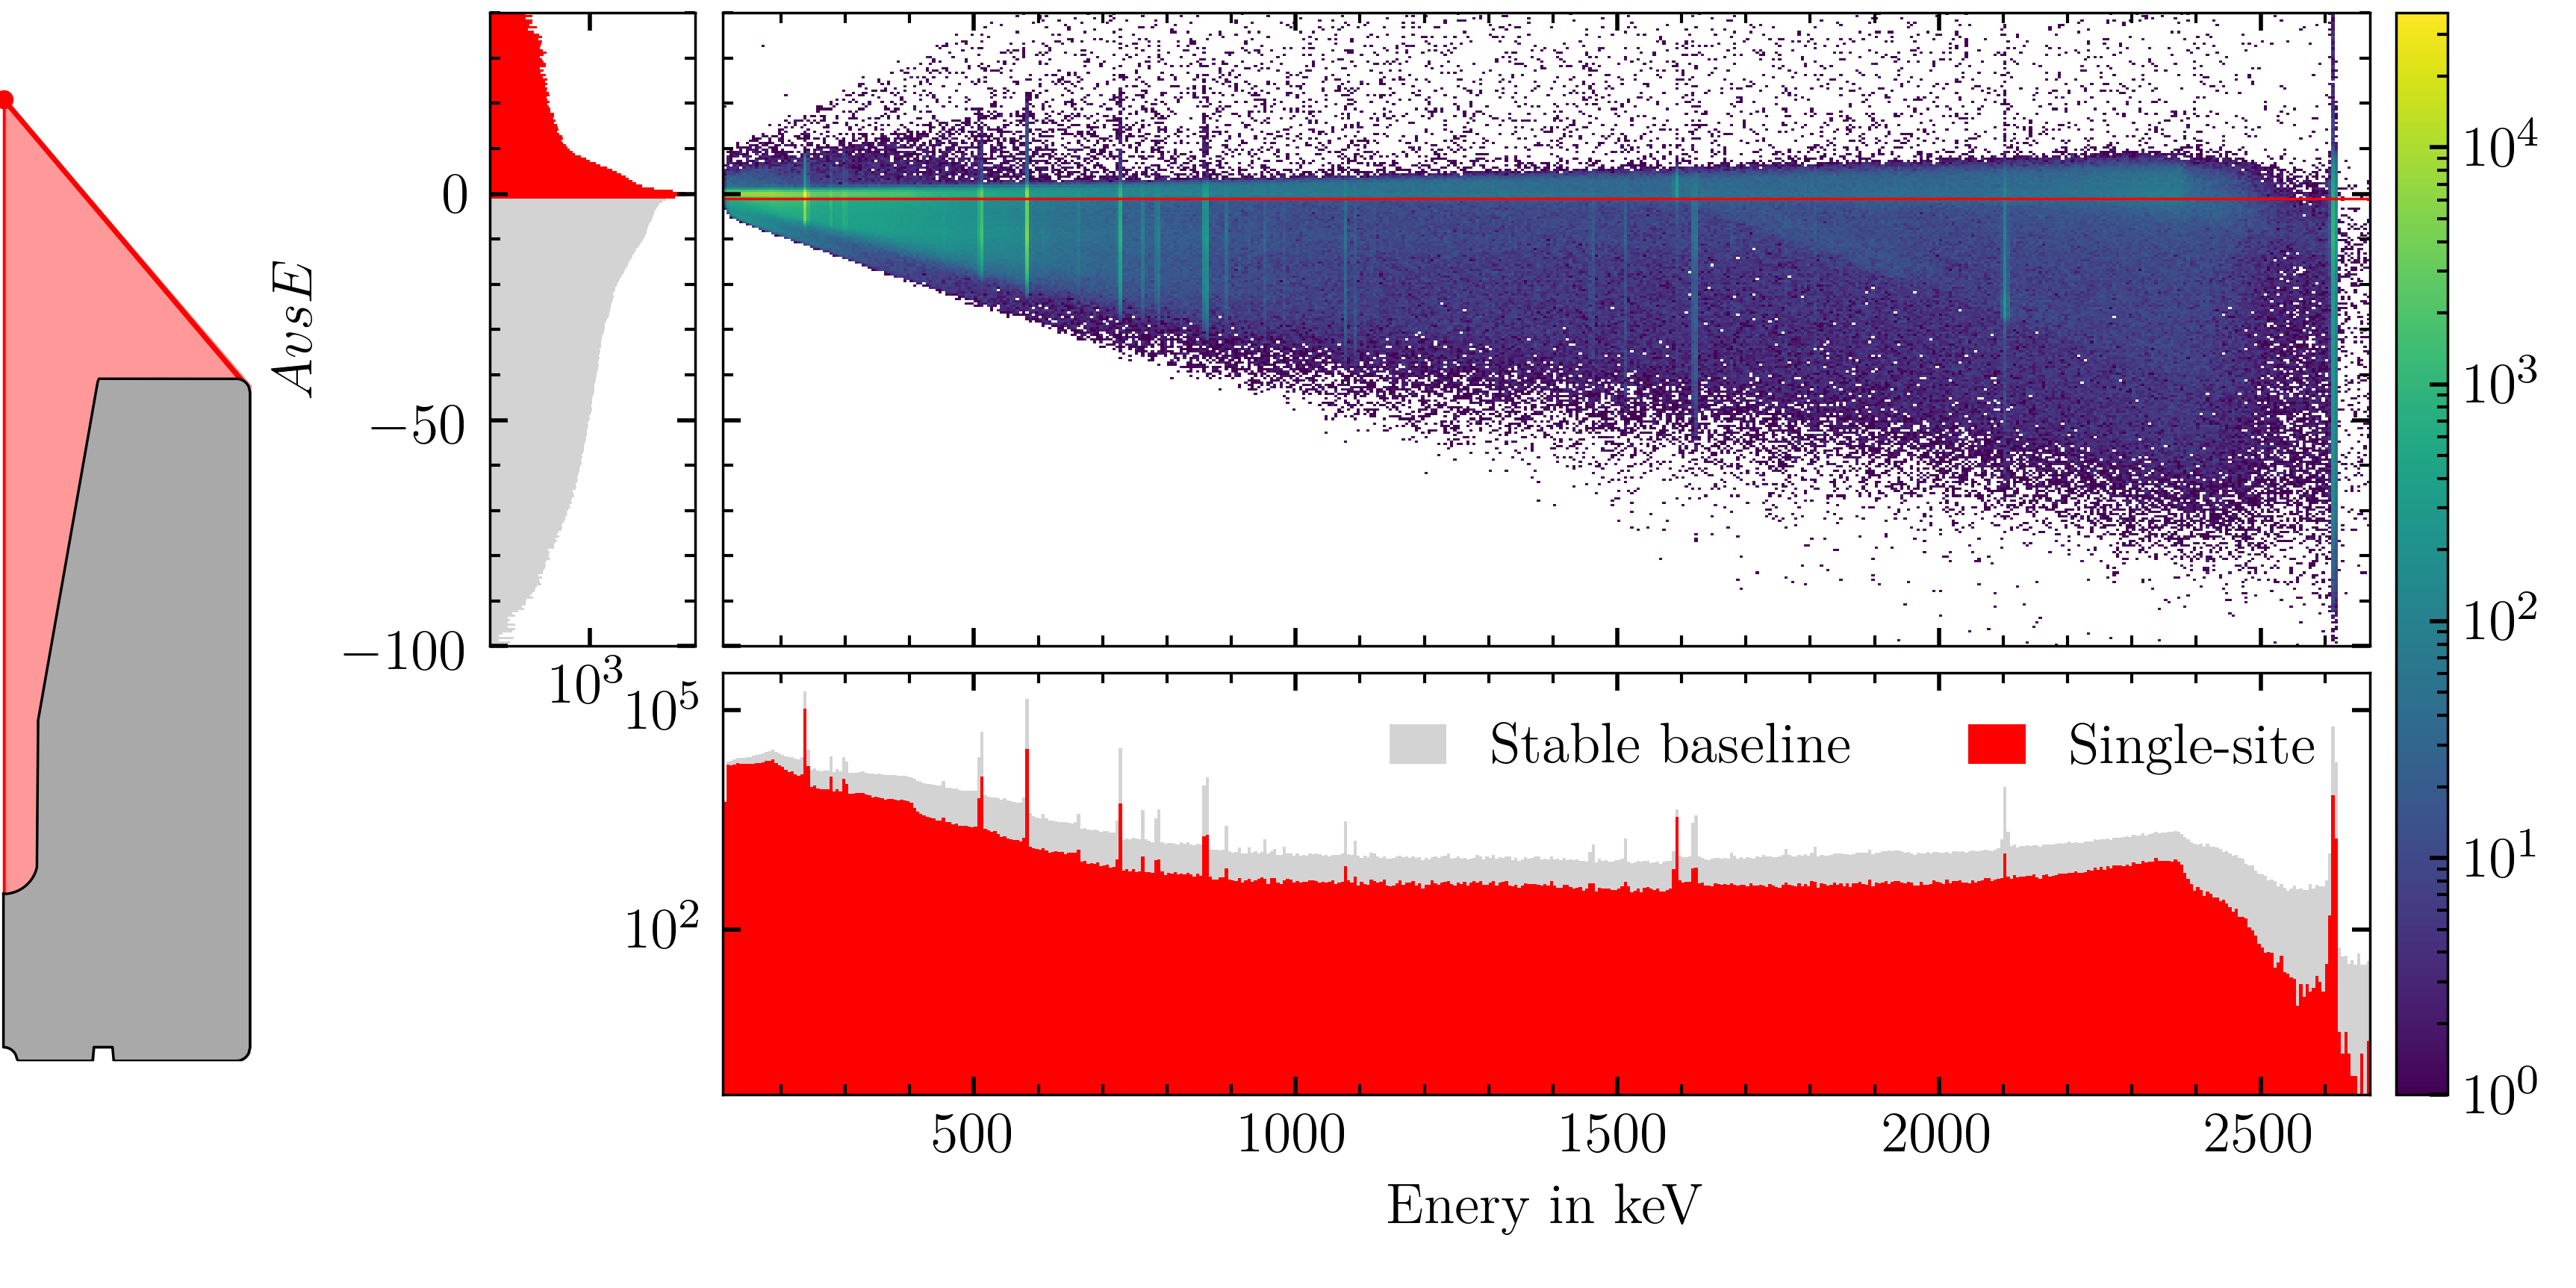
\includegraphics[width=6in]{figs/param/avse_cut.png}
    \caption{$AvsE$ is shown in relation to $E$ for resting baseline events. A red line is drawn at the cut value of -1. Events above this line are classified as single-site and shaded in red in the marginalized $E$ and $AvsE$ distributions. Most DEP and SEP events are clearly above and below this line respectively. The effect of the cut on these peaks is clearly seen in the spectrum in the bottom panel. A zoom in of the double- and single-escape peaks is shown in Fig.~\ref{fig:avse_cut_peaks}.}
    \label{fig:avse_cut}
\end{figure}
\begin{figure}[htb]
    \centering
    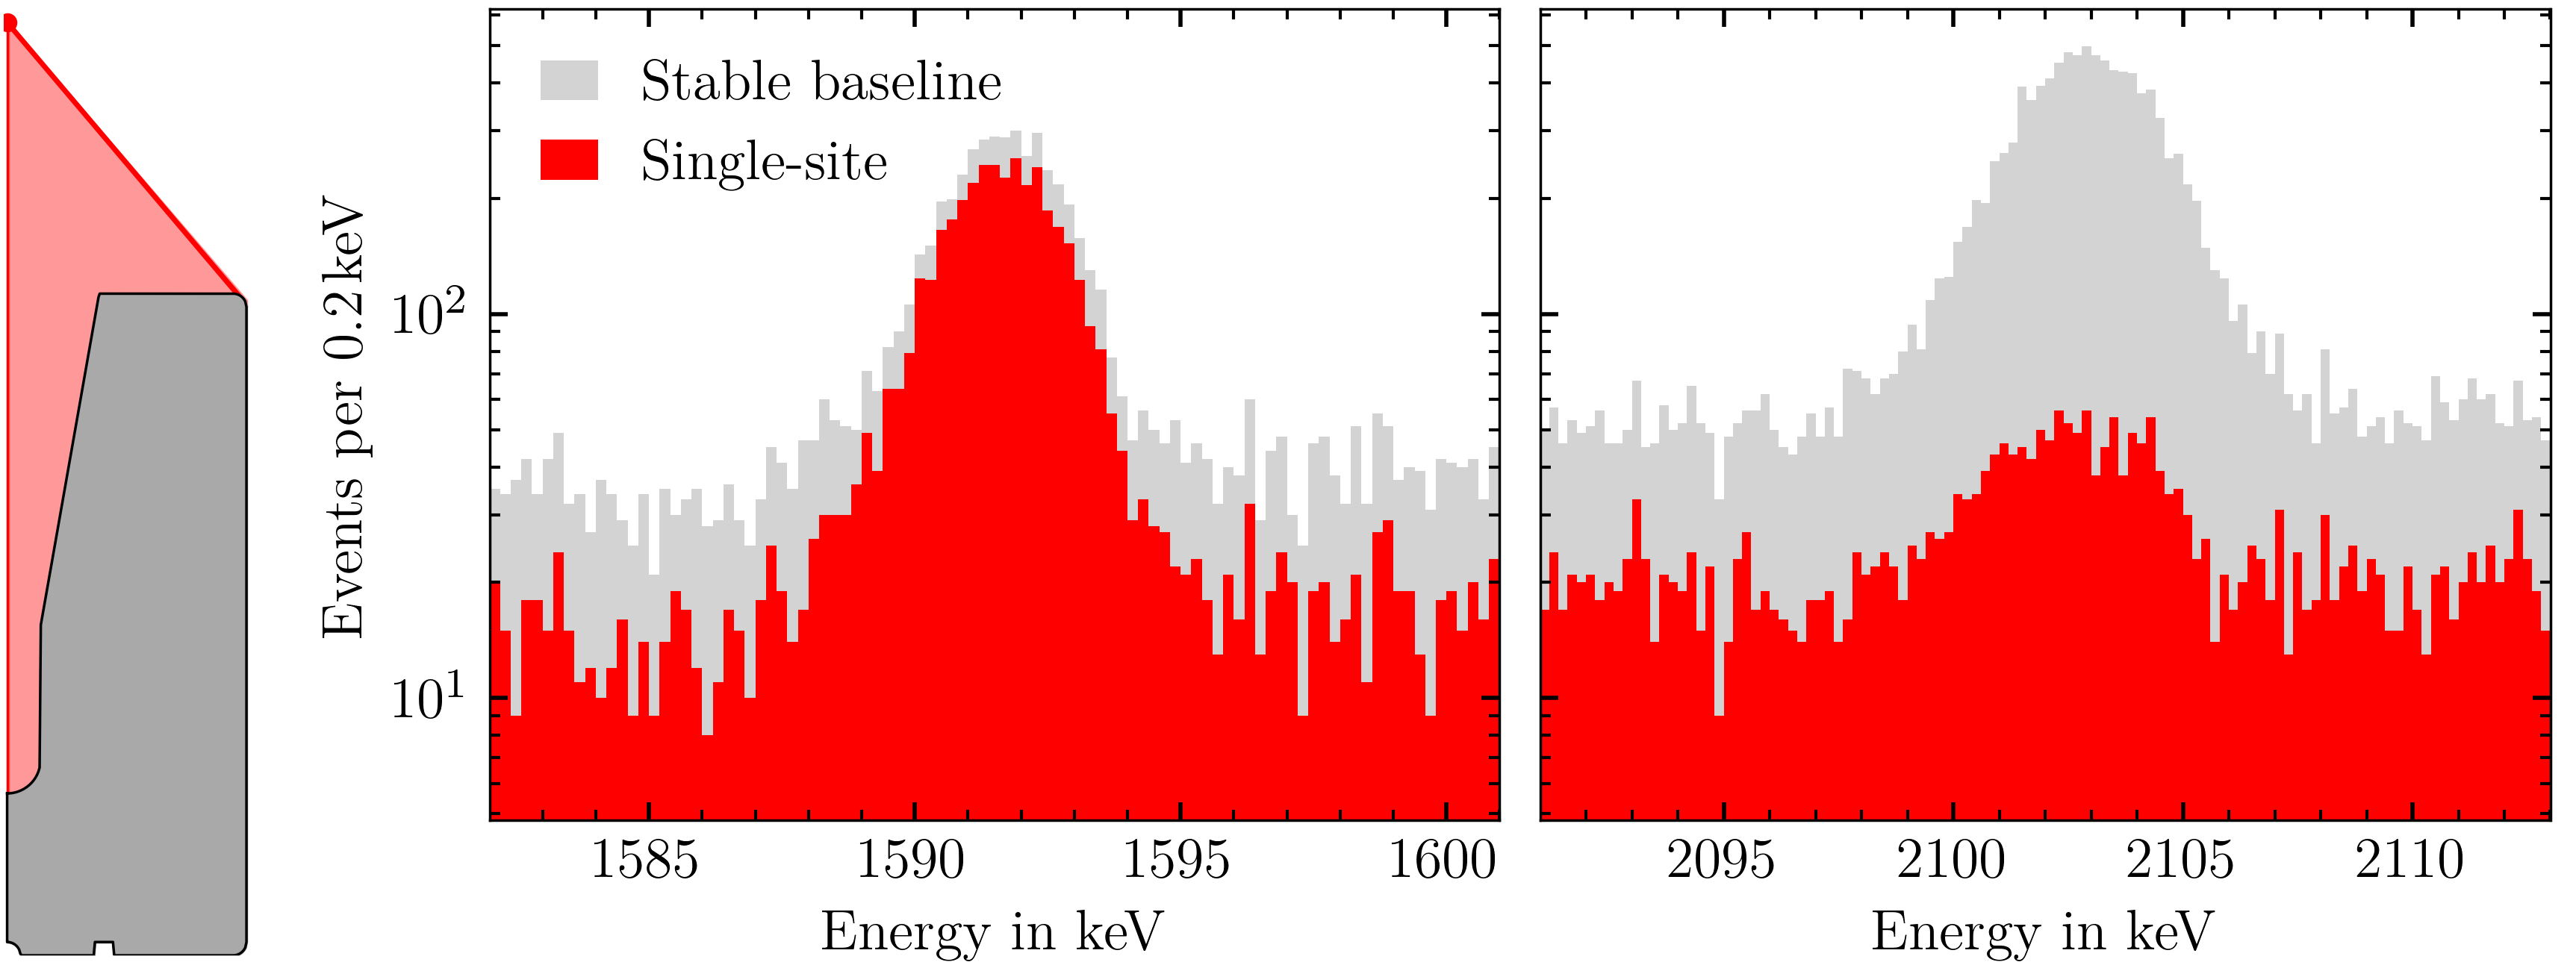
\includegraphics[width=6in]{figs/param/avse_escape_peaks.png}
    \caption{The $AvsE$ cut survival for the double- and single-escape peak survival is shown on the left and right respectively.}
    \label{fig:avse_cut_peaks}
\end{figure}

Two methods for obtaining current waveforms were considered: a first degree differentiating Savitzky-Golay (DSG) filter\footnote{A DSG filter performs a polynomial fit of the desired order to a moving window and extracts the derivative from this fit.} and a symmetric trapezoidal filter with flat time equal to zero. $A$ was calculated by performing a parabolic fit to the maximum of the current waveform and a point on each side. A range of evaluation windows and rise times were considered for the DSG and trapezoidal filters. The highest $AvsE$ SEP event rejection was obtained with a DSG filter with an evaluation window of 92\,ns. This evaluation window matched the rise plus fall time of the best performing trapezoidal filter. A single- and multi-site waveform, with their respective DSG filtered outcomes, are shown in Fig.~\ref{fig:avse_calculation}. $AvsE$ was constructed with optimal DSG filter $A$, and the fit shown in Fig.~\ref{fig:avse_calculation} in accordance with Eq.~\ref{eq:avse}. The resulting distribution is shown in Fig.~\ref{fig:avse_cut}.

To count the number of DEP and SEP events, sideband background subtraction was used: the number of peak events is equal to the number of events falling in the peak region minus one fourth the number of events falling in regions twice as wide on each side of the peak region. To tune the cut, the 10$^\text{th}$ percentile of the DEP was calculated by integrating over the peak and sideband regions appropriately. The 10$^\text{th}$ percentile set the cut tuning value $j$, resulting in the desired 90\% DEP event survival.

The process of fitting $A_\text{cal}$, and constructing and tuning $AvsE$ is conducted separately for resting baseline and soft pileup events. A similar SEP and \novbb{} continuum acceptance is obtained. These results are summarized in Tab.~\ref{tab:avse_survival}. Note that soft pileup $AvsE$ uses $E_\text{RSC}$. A 4\% higher acceptance of the SEP was obtained when constructing $AvsE$ with the uncorrected energy. The \novbb{} continuum (\Qbb{} $\pm$ 50\,keV) is used as a proxy for a Compton dominated region. The performance of $AvsE$ is further evaluated in the \CsS{} Compton continuum in Sec.~\ref{subsec:singlesitecompton}. 
\begin{table}[tbph]
    \centering
    \caption{Summary of DEP, SEP and \novbb{} continuum acceptance for resting baseline and soft pileup events.}
	\vspace{12pt}
	\begin{tabularx}{1\textwidth}{>{\tr}X >{\tr}X >{\tr}X}
		\hline \noalign{\vskip 1ex}
		Energy region & Resting baseline accept. in \% & Soft pileup accept. in \%\\[1ex]
		\hline \noalign{\vskip 1ex}
		DEP & 90.0 & 90.0\\
		SEP & 7.7 & 8.0\\
		\novbb{} continuum & 39.2 & 40.2\\[1ex]
		\hline
	\end{tabularx}
	\label{tab:avse_survival}
\end{table}